%% ****** Start of file apssamp.tex ******
%
%   This file is part of the APS files in the REVTeX 4.1 distribution.
%   Version 4.1r of REVTeX, August 2010
%
%   Copyright (c) 2009, 2010 The American Physical Society.
%
%   See the REVTeX 4 README file for restrictions and more information.
%
% TeX'ing this file requires that you have AMS-LaTeX 2.0 installed
% as well as the rest of the prerequisites for REVTeX 4.1
%
% See the REVTeX 4 README file
% It also requires running BibTeX. The commands are as follows:
%
%  1)  latex apssamp.tex
%  2)  bibtex apssamp
%  3)  latex apssamp.tex
%  4)  latex apssamp.tex
%
\documentclass[%
 reprint,
%superscriptaddress,
%groupedaddress,
%unsortedaddress,
%runinaddress,
%frontmatterverbose, 
%preprint,
%showpacs,preprintnumbers,
%nofootinbib,
%nobibnotes,
%bibnotes,
 amsmath,amssymb,
 aps,
 nofootinbib
%pra,
%prb,
%rmp,
%prstab,
%prstper,
%floatfix,
]{revtex4-1}

\usepackage{color}
\usepackage{graphicx}
\usepackage[caption=false]{subfig}
\usepackage{graphicx}% Include figure files
\usepackage{dcolumn}% Align table columns on decimal point
\usepackage{bm}% bold math
\usepackage{graphicx}% Include figure files
\usepackage{dcolumn}% Align table columns on decimal point
\usepackage{bm}% bold math
%\usepackage{hyperref}% add hypertext capabilities
%\usepackage[mathlines]{lineno}% Enable numbering of text and display math
%\linenumbers\relax % Commence numbering lines

%\usepackage[showframe,%Uncomment any one of the following lines to test 
%%scale=0.7, marginratio={1:1, 2:3}, ignoreall,% default settings
%text={7in,10in},centering,
%%margin=1.5in,
%%total={6.5in,8.75in}, top=1.2in, left=0.9in, includefoot,
%%height=10in,a5paper,hmargin={3cm,0.8in},
%]{geometry}


\newcommand{\bra}[1]{\langle#1|}
\newcommand{\ket}[1]{|#1\rangle}
\newcommand{\braket}[2]{\langle#1|#2\rangle}
\newcommand{\bracket}[3]{\langle#1|#2|#3\rangle}
\newcommand{\Eval}[1]{\langle#1\rangle}
\newcommand{\op}[2]{|#1\rangle\langle#2|}
\newcommand{\pd}[1]{\frac{\partial}{\partial #1}}
\newcommand{\Pd}[2]{\frac{\partial #1}{\partial #2}}
\newcommand{\pdd}[1]{\frac{\partial^2}{\partial #1^2}}
\newcommand{\D}{\Delta}
\newcommand{\g}{\gamma}
\newcommand{\Om}{\Omega}
\newcommand{\om}{\omega}
\newcommand{\ve}[1]{\mathbf{#1}}
\newcommand{\ved}[1]{\mathbf{e}_{#1}}
\newcommand{\dd}[1]{\frac{\text{d}}{\text{d}t}}
\newcommand{\dive}[1]{\nabla\cdot #1}
\newcommand{\curl}[1]{\nabla\times #1}

\newcommand{\lr}[1]{\left(#1\right)}
\newcommand{\lrs}[1]{\left[#1\right]}

\newcommand{\diag}{\text{diag}}

\newcommand{\sech}{\text{sech}}
%\newcommand{\tanh}{\text{tanh}}

\newcommand{\al}[1]{
\begin{eqnarray}#1\end{eqnarray}
}
 % for Jessie

\begin{document}

%\preprint{APS/123-QED}

\title{Scattering in atomic and molecular physics \\ AM205 Final Project}% Force line breaks with \\
% \thanks{A footnote to the article title}%

\author{Ben Augenbraun, Andrei H. Gheorghe, Jessie T. Zhang}

\date{\today}% It is always \today, today,
             %  but any date may be explicitly specified

\begin{abstract}
The study of collisions between pairs of atoms or molecules represents a vibrant subfield of atomic, molecular, and optical (AMO) physics. Theoretical physicists have invested a large amount of effort toward understanding these collisions ranging from physical chemistry experiments in the lab to astrophysical observations. Here, we review and implement several approaches to solve atomic and molecular scattering problems which, together, allow us to explore a wide range relevant parameters. In particular, we apply fully classical, semi-classical, and fully quantum mechanical algorithms to these scattering problems. Our methods and results are discussed in detail, demonstrating good agreement with experimental results and physical intuition.
\end{abstract}

\maketitle

\section{\label{sec:Introduction}Introduction}
It is the opinion of most physicists that simple questions deserve simple answers. Nevertheless, the (seemingly) simple question of, ``what happens when atom (or molecule) X collides with atom (or molecule) Y?" is not a simple one to answer. Nearly immediately after the discovery of quantum mechanics, physicists sought to describe the basic structure of matter within a quantum formalism. Broadly speaking, they did this by comparing theoretical predictions with experimental observations in one of two ways: by studying the precise internal structure of isolated atoms or molecules, or by studying the interactions between atoms and molecules~\cite{SchrodPaper1926,DiracTextbook,QuantumScatteringTextbook}. In order to isolate the atom or molecule under study from environmental perturbations, these studies were (and still are) often undertaken in highly dilute gas phases. In such cases, the density is low enough that the most likely sort of interaction is a collision between just a pair of particles. Even in these binary interactions, a great deal of physics lurks: (a) the collision can redistribute energy between the collision partners; (b) the internal quantum state of one, or both, of the colliding particles can be changed; and (c) it is possible that a chemical reaction occurs in which the very makeup of the collision complex changes from beginning to end.

\subsection{Physical Motivation}
Each of these three broad classes of collisions is of physical relevance to one or another subfield of physics. For example, detailed understanding of collision processes is of great importance to astrophysics because collisions are one of the main processes which can alter the rotational and vibrational internal states of molecules in interstellar clouds of dust~\cite{ColdChemBook,ColdMolsBook}. Once a collision has excited rotational or vibrational motions in the molecular constituents of the interstellar medium, excited-state molecules inevitably decay back to their ground states, emitting electromagnetic radiation in the process. Therefore, estimating the abundances and species of molecules present in outer space by studying the spectral lines observed by telescopes requires accurate \textit{a priori} knowledge of collisional rate coefficients~\cite{ColdChemBook}. Though over a hundred molecular species (including complex organic molecules) have been observed in space, most abundant in interstellar space are the ``simple" species of H, He, and H$_2$. Hence, many theoretical investigations of collisional processes for astrophysical purposes include collisions with these species. Furthermore, these collision calculations are often performed at temperatures ranging from a few Kelvin (K) to many tens of K, to match the typical temperatures observed in interstellar space. An example of such a calculation is provided in Sec.~\ref{sec:QuantumMethod}. For later reference, we will refer the temperature range on the order of a few Kelvin as ``cold."

At lower, so-called ``ultracold" temperatures ($< 1$ mK), temperatures much colder than even that of outer-space, collisions remain important to atomic and molecular physicists working in the laboratory. It is actually a surprising truth that, even at temperatures approaching absolute zero, the interactions between atoms and molecules in dilute gases remain rich--- rather than simply ``freezing out" as the thermal motion approaches stand-still. In fact, the last two decades have seen tremendously exciting research on the use of laser cooling to reduce the temperatures of atomic gases to just fractions of a degree above absolute zero. Perhaps the crowning achievement of this work was the realization of Bose-Einstein condensation, a phase transition to a fully new form of matter in which the quantum, wave-like nature of the constituent particles takes over and a gas of millions or even billions of atoms ceases to have identifiable constituent particles. The achievement of this goal was made possible by two inventions: laser cooling and evaporative cooling. Laser cooling, though broadly applicable and efficient, typically only produces temperatures around a few hundred $\mu$K. The technique of ``evaporative cooling" has allowed researchers to produce gases nearly six orders of magnitude colder ($\sim$1 nK). The idea is simple: one takes a trapped sample of atoms, removes the hottest ones, and then waits for collisions between the remaining atoms to thermalize the gas at a new, lower average energy. This process is reminiscent of how one might attempt to cool a hot cup of tea by blowing on it. Importantly, the evaporation scheme is only possible if  ``good" elastic collisions, which lead to re-thermalization and cooling, predominate over ``bad" inelastic collisions, which can lead to heating and trap loss. If collisions are to be used as a tool in this scheme, it is highly important to be able to predict which species are most amenable to the evaporation. That is, which species have high ratios of elastic to inelastic collision rates. In this way, theoretical predictions about scattering properties guide experiments to success.

\subsection{Theoretical Methods in Scattering Theory}

Based on this motivations, theoretical physicists have focused much effort on a complete description of a general collision process. In this paper, the problem we set out to solve is how to describe atomic and molecular collisions accurately. We focus on three potential methods, each of which is widely used by professional theorists. One, classical trajectory tracking, neglects quantum mechanical effects and simply asks: what orbits do colliding atoms and molecules take? By running many individual trajectories and looking at the statistics of these collisions, one can extract experimentally useful parameters such ask collision lifetimes and reaction rates. Furthermore, this method allows us to examine the role that chaos may play in atom + molecule collisions, especially at the ultralow temperatures commonly studied in experiments. Another method, called the RRKM method, attempts to use a mix of semi-classical and quantum mechanical reasoning to ascertain statistics about the collisions. In particular, the potential energy surface is treated semi-classically and solved for as a single channel problem quantum mechanically. Finally, we also consider fully quantum mechanical solutions of the scattering problem. This involves solving a Schrodinger equation including interaction potentials defined by the collision partners. While this is surely the most ``complete" description of a collision attainable, it is also the most difficult: not only can the Schrodinger equation considered include many coupled collision channels, but without sufficiently accurate interaction potentials the solution to the problem will not match reality. Determining these potential energy curves is a full-fledged field of theoretical physics in its own right, and one which we do not explore here. Instead, we study algorithms to solve the quantum scattering problem using toy potentials. In this way, we can extract collision properties in line with physical intuition but not highly accurate for any particular system. Note that, throughout this paper, we follow the standard convention that energy and temperature are considered somewhat equivalent here and are related by $E = k_B T$, where $k_B$ is Boltzmann's constant. We also make use of atomic units, in each $\hbar = 1$ and the unit of energy if the Hartree.\footnote{The abbreviation for ``atomic units" is a.u., and should not be confused with arbitrary units.}


\section{\label{sec:ClassicalTraj} Classical Method: Trajectory Tracking}

Due to the large number of available rovibrational states, doing a full multi-channel quantum mechanical study of a reaction between even a single atom and a single dimer is beyond the scope of this project. Indeed, only recently have professional theorists tackled such problems. However, as observed by Croft and Bohn~\cite{bohn2014}, many of the features and observables of a collision between an atom and a dimer, such as its chaotic behavior or scattering rate, can be computed by using a purely classical approach. This poses a much more computationally tractable problem. Furthermore, even though the collision problem is quantum at its core, in the midst of a collision--- deep inside the potential energy wells of the Lennard-Jones potential, for instance--- the particles' kinetic energies are actually quite large, putting them in a regime where one might expect classical reasoning to be a good approximation. Ultimately, however, it is only the accuracy with which the results reflect physical reasoning and experimental results that determines their applicability.

Here, we report on classical trajectory tracking of atom + dimer collisions in order to extract information about the complex interactions between these particles. This is of experimental relevance because during a collision the particles become ``dark" to the experimentalist: they can no longer be observed spectroscopically due to large perturbations in their energy levels, and they may also therefore leave any external traps in which the initial particles were confined. Only if the collision lifetime is sufficiently short will the particles survive the collision still in the experimental setup. Otherwise, there will be detectable losses from the apparatus. Interpreting these losses is tricky, because many processes can cause loss. Hence, accurate models of the losses as a function of collision energy and other variables are important for interpreting data. Our results below represent one such analysis.

\subsection{\label{sec:level2}Computational method}

To perform the classical computation we assume that the interaction is purely determined by a pairwise-additive Lennard-Jones potential

\begin{equation}
U(\mathbf{r_{\mathrm{1}}}, \mathbf{r_{\mathrm{2}}}, \mathbf{r_{\mathrm{3}}}) = \sum_{i \neq j} \frac{C_{\mathrm{12}}}{(\mathbf{r_{\mathrm{i}}}-\mathbf{r_{\mathrm{j}}})^{12}} - \frac{C_{\mathrm{6}}}{(\mathbf{r_{\mathrm{i}}}-\mathbf{r_{\mathrm{j}}})^6},
\label{eq:LJ}
\end{equation}
\noindent where $C_{\mathrm{6}}$ is the leading order van der Waals coefficient, and the higher order $C_{\mathrm{12}}$ is chosen in order to obtain the correct atom-atom well depth, as given by $D_{\mathrm{e}} = C_{\mathrm{6}}^2/4D_{\mathrm{e}}$.  The values of the van der Waals coefficients used are summarized in Table~\ref{table:coeffs}, where the atomic species are chosen to span a wide range of experimentally viable choices. Other effects such as contributions due to the spin of the atoms are ignored. 

\begin{table}
\begin{center}
 \begin{tabular}{|c c c|} 
 \hline
 System & C6 (a.u.) & C12 (a.u.)\\ 
 \hline\hline
$\text{Li} + \text{Li}$ & 1394 & 1521.8e-6 \\ 
 \hline
 $\text{Cs} + \text{Cs}$ & 6891 & 1271.2e-6 \\
 \hline
\end{tabular}
\caption{$C_6$ Van der Waals coefficients and well depths $D_e$ for $\mathrm{Li_2}$~\cite{dattani2011} and $\mathrm{Cs_2}$~\cite{xie2009}.}
\label{table:coeffs}
\end{center}
\end {table}

An exaggerated version of the Lennard-Jones potential is given in Fig.~\ref{fig:schematic}, together with the basic setup of the collision's initial conditions. We thus distinguish the orientation of the dimer in the XZ-plane, $\theta_0$, the initial velocity of the incoming atom (in the rest frame of the dimer), as given by the initial temperature $T$, and the impact parameter, $b$, as some of the initial condition variables we can tune in order to analyze the collision. As already mentioned, we can also consider different atomic species, which changes the masses and the interaction strengths.

\begin{figure}[htp]
\subfloat{
  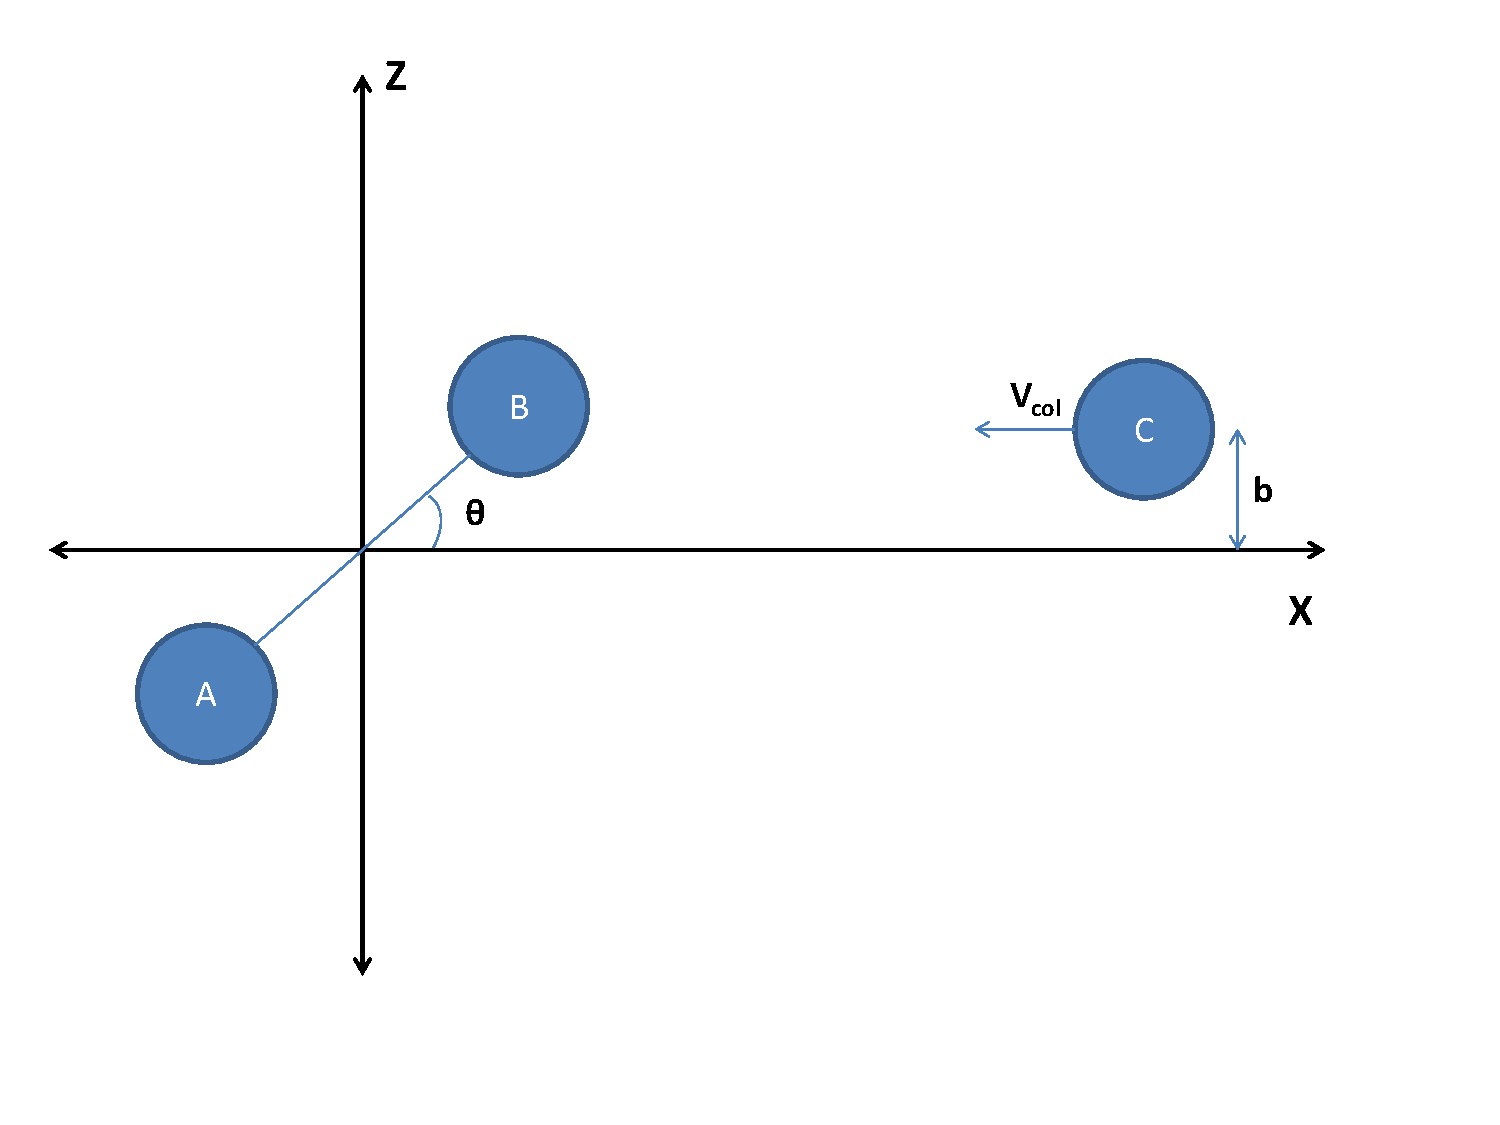
\includegraphics[clip,width=1\columnwidth]{schematic.pdf}%
}

\subfloat{
  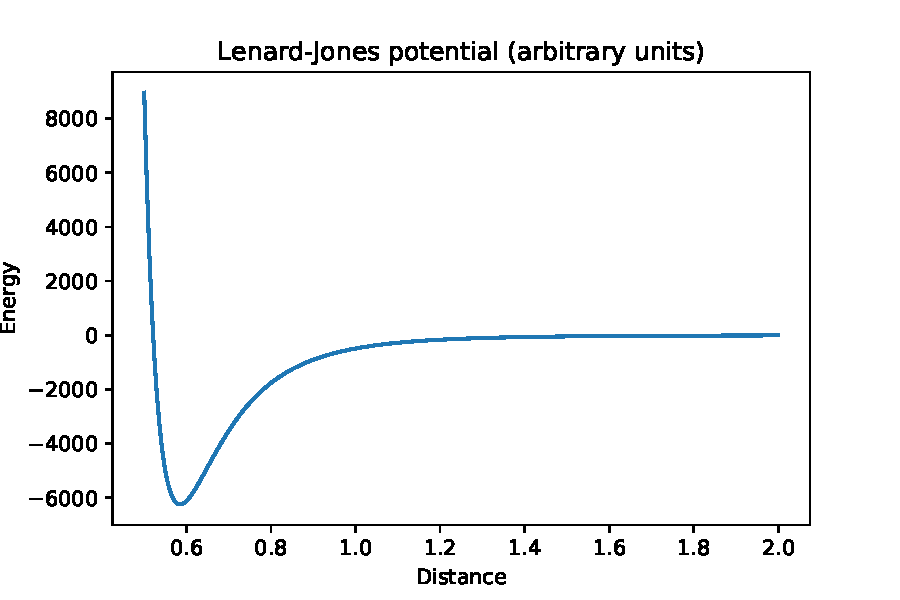
\includegraphics[clip,width=1\columnwidth]{LJ.pdf}%
}

\caption{Top: Schematic of atom-dimer collision, including all the initial conditions variables. Bottom: Model of Lennard-Jones atom-atom pair potential.}
\label{fig:schematic}
\end{figure}

 We numerically integrate the classical trajectories according to the following algorithm (the code this describes can be found in $\texttt{molecCollPackage.py}$). For a particular choice of atom + dimer, we define analytically the derivatives of the Lennard-Jones potential to compute the force acting on each atom: $\mathbf{F} = -\mathbf{\nabla}V$. It is assumed that the dimer starts at the origin with zero kinetic energy, and the lone atom approaches along the $x$-axis with kinetic energy set by the initial temperature, initially displaced far enough that it feels a vanishingly small force from the dimer. We also specify an initial angle of the dimer relative to the collision axis, and an impact parameter to offset the colliding atom from the collision axis. We then transform into the center-of-mass frame by boosting at a velocity equal to $1/3$ of the incoming atom's velocity. Using a $\texttt{scipy}$ integration routine, we then propagate each atom under the influence of the Lennard-Jones potentials until the collision complex has broken apart. We determine the time at which this happens based on when the hyperradius of the complex, defined by $r_\text{hyp} = \sqrt{r_{AB}^2 + r_{AC}^2 + r_{BC}^2}$, exceed the initial distance between the atom and dimer. The total time between the beginning of the simulation and the time at which we claim the collision has broken apart is called the lifetime of the collision. For certain statistics which will be described in detail below, it is also important to know more than just the collision lifetime. Therefore, we also record which atom(s) emerge from the collision as a lone atom, and which as part of a dimer. We thereby assign each collision to a ``basin" defined by which atom emerges alone.

We have tried a variety of numerical integrators and have found that variable step-size integrators such as $\texttt{DOP853}$ perform reasonably. We have varied the maximum step size to ensure our results are convergent, which was tested by doubling the maximum step size and making sure that none of the collision statistics changed. The figures presented below are all based on parameter choices that satisfied this condition. To check the dependence of the collision on infinitesimal changes to, e.g., the dimer initial angle we have also written code which runs two collisions differing only by a small variation in this initial angle. As is described below, this is a useful way to test for the emergence of chaotic behavior in the system. When necessary, we have run this code on the Odyssey computing cluster in order to speed up evaluation time for the large numbers of averages we computed in the results below.


\begin{figure}[htp]
\subfloat{
  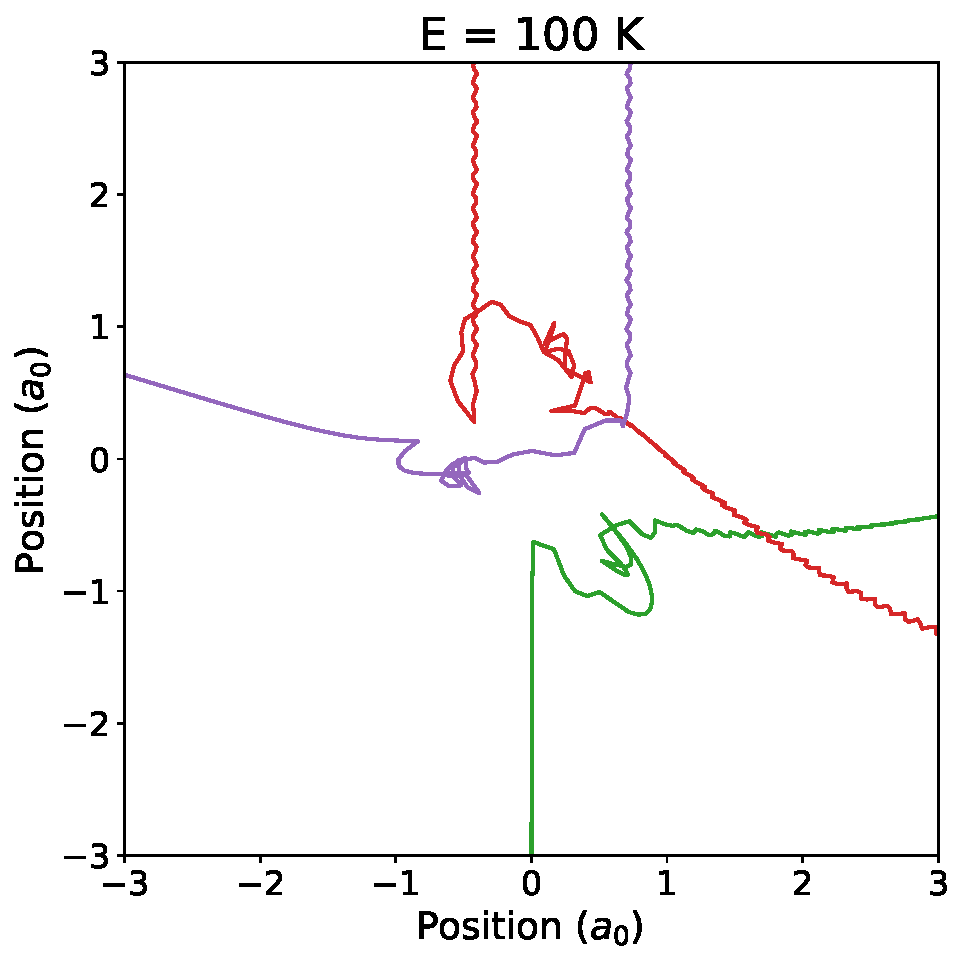
\includegraphics[clip,width=0.85\columnwidth]{Col100K.pdf}%
}

\subfloat{
  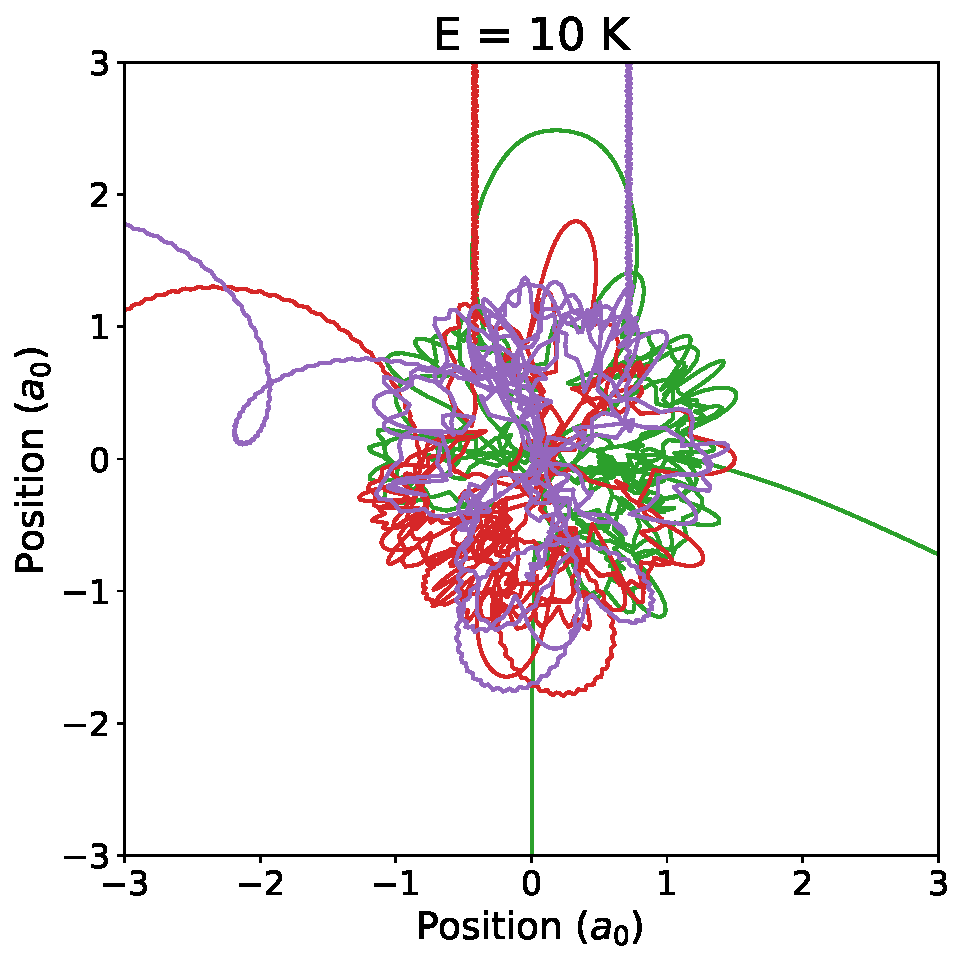
\includegraphics[clip,width=0.85\columnwidth]{Col10K.pdf}%
}

\subfloat{
  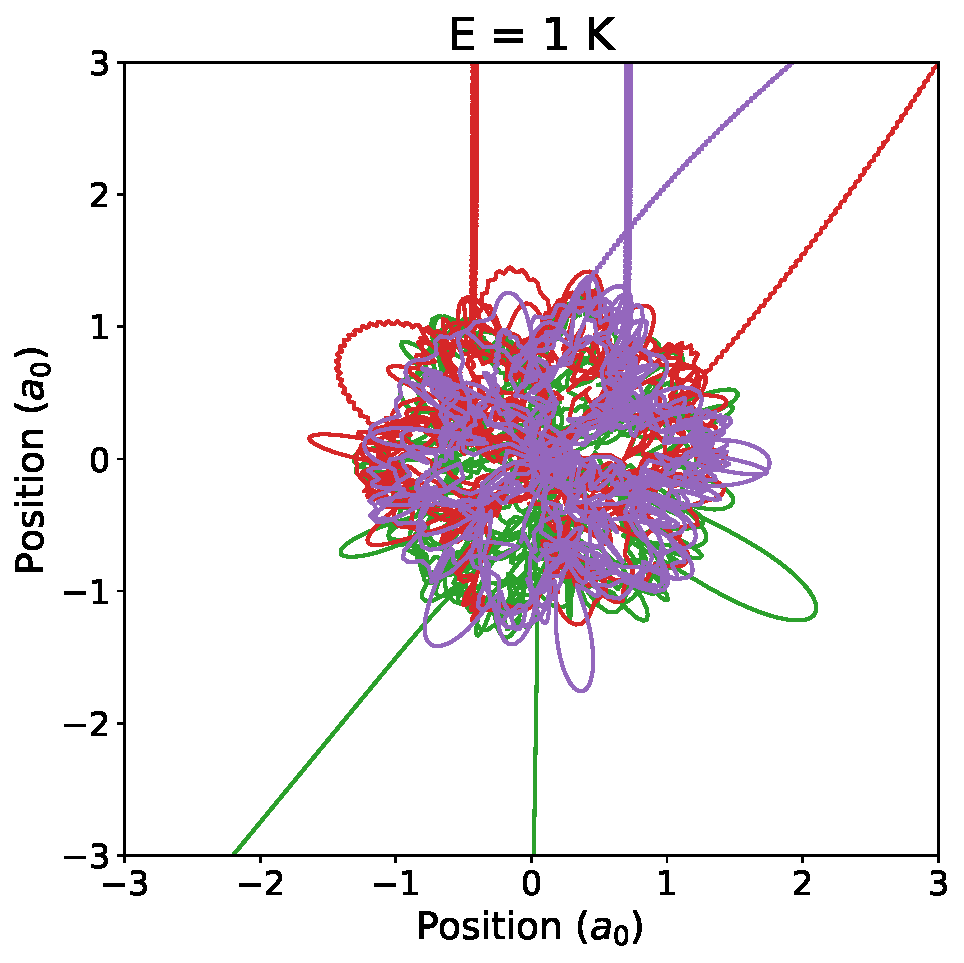
\includegraphics[clip,width=0.85\columnwidth]{Col1K.pdf}%
}

\caption{Three example collision trajectories in the center-of-mass frame. As the energy is lowered, the orbit becomes increasingly complex and increasingly long-lived.}
\label{fig:collisioncomplexes}
\end{figure}

\subsection{\label{sec:level2}Collision-Complex Lifetime}
One of the main observables of interest in ultracold collisions is the complex's lifetime (or the related quantity of scattering rate), which can provide information about the ergodicity of the reaction and can also be used as an observable to test different models of the collsion. As described previously, it is also an important parameter when the only sign of a collision is trap loss. Note that in Sec.~\ref{sec:RRKM} we describe semi-classical treatments of the collision lifetime problem. Here, however, we focus on wholly classical analysis. To this end, we compute the lifetime of the reaction as the time between the initial starting point\footnote{The atom starts $r_{\mathrm{init}} = 60 a_0$ away from the dimer, where $a_{\mathrm{0}}$ is the Bohr radius and the equilibrium distance between the dimer's atoms is $\bar{a} = 8.78 a_{\mathrm{0}}$.} and the time when the hyper-radius $\sqrt{r^2_{\mathrm{AB}} + r^2_{\mathrm{BC}} + r^2_{\mathrm{AC}}}$ is first greater than $ r_{\mathrm{init}}$. We note that different methods of timing the reaction are possible, but they should not change the functional behavior of the lifetime. In Fig.~\ref{fig:collisioncomplexes} we show sample trajectories at a variety of collision energies. As the collision energy is decreased, a marked increase in complexity of the orbits arises. We can analyze this more carefully by running many sets of collisions and studying the complex's lifetime as a function of temperature. In particular, we analyze this for two atomic species, as shown in Fig.~\ref{fig:lifetime}. Each point represents the average of 500 individual trajectories. We observe that lifetime has a power-law dependence on the initial energy, with exponent $-0.47$ for $\mathrm{Li} + \mathrm{Li_{2}}$ and $-0.50$ for $\mathrm{Cs} + \mathrm{Cs_{2}}$. 

One explanation for why the lifetime of the collision complex increases as the collision energy decreases is that, at low collision energies the particles are initially accelerated into the well of the Lennard-Jones potential, and when they are in near proximity to one another they undergo a large number of ``mini" collisions which effectively randomizes the distribution of energies between the three individual atoms. Only a very small number of these distributions actually leads to the complex breaking apart, and therefore the atoms can spend a long time orbiting each other before this happens. At high collision energies, it is much easier for an individual atom to ``find a way" to escape, which leads to short lifetimes in that extreme. 

\begin{figure}[ht]
\begin{center}
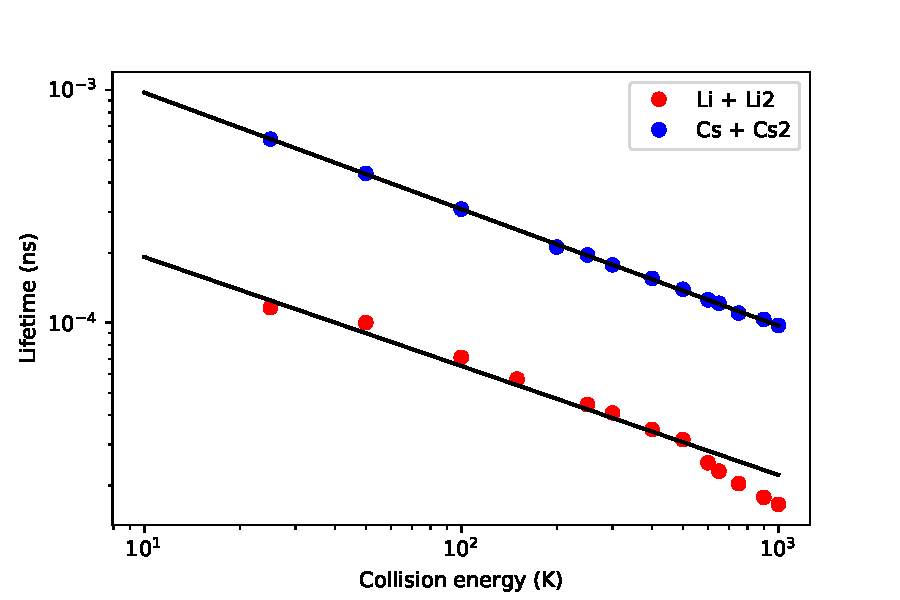
\includegraphics[width=1.1\linewidth]{lifetime.pdf}
\caption{Lifetime as a function of the collision energy for the atom-dimer cases of $\text{Li} + \text{Li}_2$ and $\text{Cs} + \text{Cs}_2$. The dots represent the computed total time that the atom-dimer pair spend in the reaction, while the solid line represents a power-law fit.}
\label{fig:lifetime}
\end{center}
\end{figure}


\subsection{\label{sec:level3}Chaos}

It has long been suggested that chaos may play a role in cold and ultracold collisions of atoms and molecules. Though our initial trajectory results certainly indicate \textit{complex} interactions, it is not yet clear whether they demonstrate \textit{chaotic} ones. Our simulations let us explore the emergence of chaos in a quantitative way as the atoms interact in low-energy regimes and the interactions become relatively more important than the initial kinetic energies. We can observe the chaotic behvaiour by analyzing the outcome of trajectories as a function of the initial conditions. We thus vary $\theta$, the angle of orientation of the dimer with respect to the velocity of the incoming atom, and look at both the lifetime of the trajectory as well at what ``kind" of trajectories they are: we use the fact that this is a classical collision and can therefore label each atom involved; we thus classify trajectories by whether the two initial atoms forming the dimer stayed together (AB+C), whether they changed partners (AC+B or BC+A), or whether the complex broke apart with all three atoms flying apart independently (A+B+C).

The results for $\mathrm{Li} + \mathrm{Li_2}$ at $T = 350~\mathrm{K}$ are summarized in Fig.~\ref{fig:chaos}. We conclude that, while there are regions of relative stability, both the lifetime and the ending ``basin" can vary wildly as a function of $\theta$. Even more compelling, by ``zooming in" on a region of $\theta$ we qualitatively observe the same features, so we conclude that the system exhibits the scale invariance characteristic of fractals.

\begin{figure}[htp]
\subfloat{
  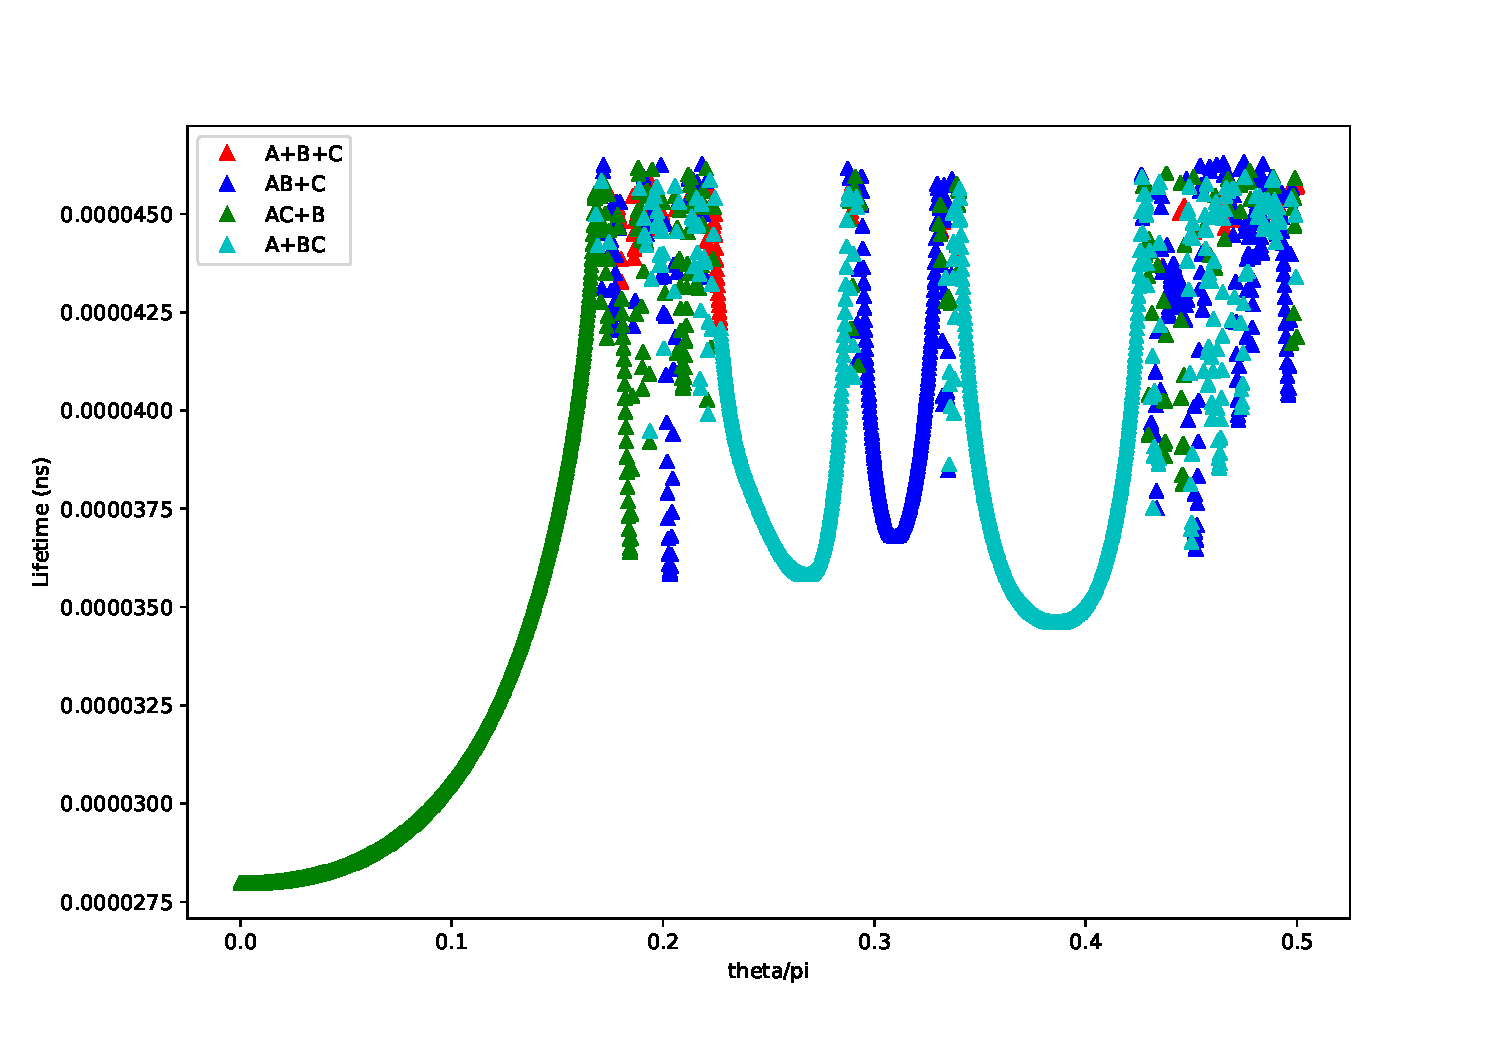
\includegraphics[clip,width=1.1\columnwidth]{fractal_big.pdf}%
}

\subfloat{
  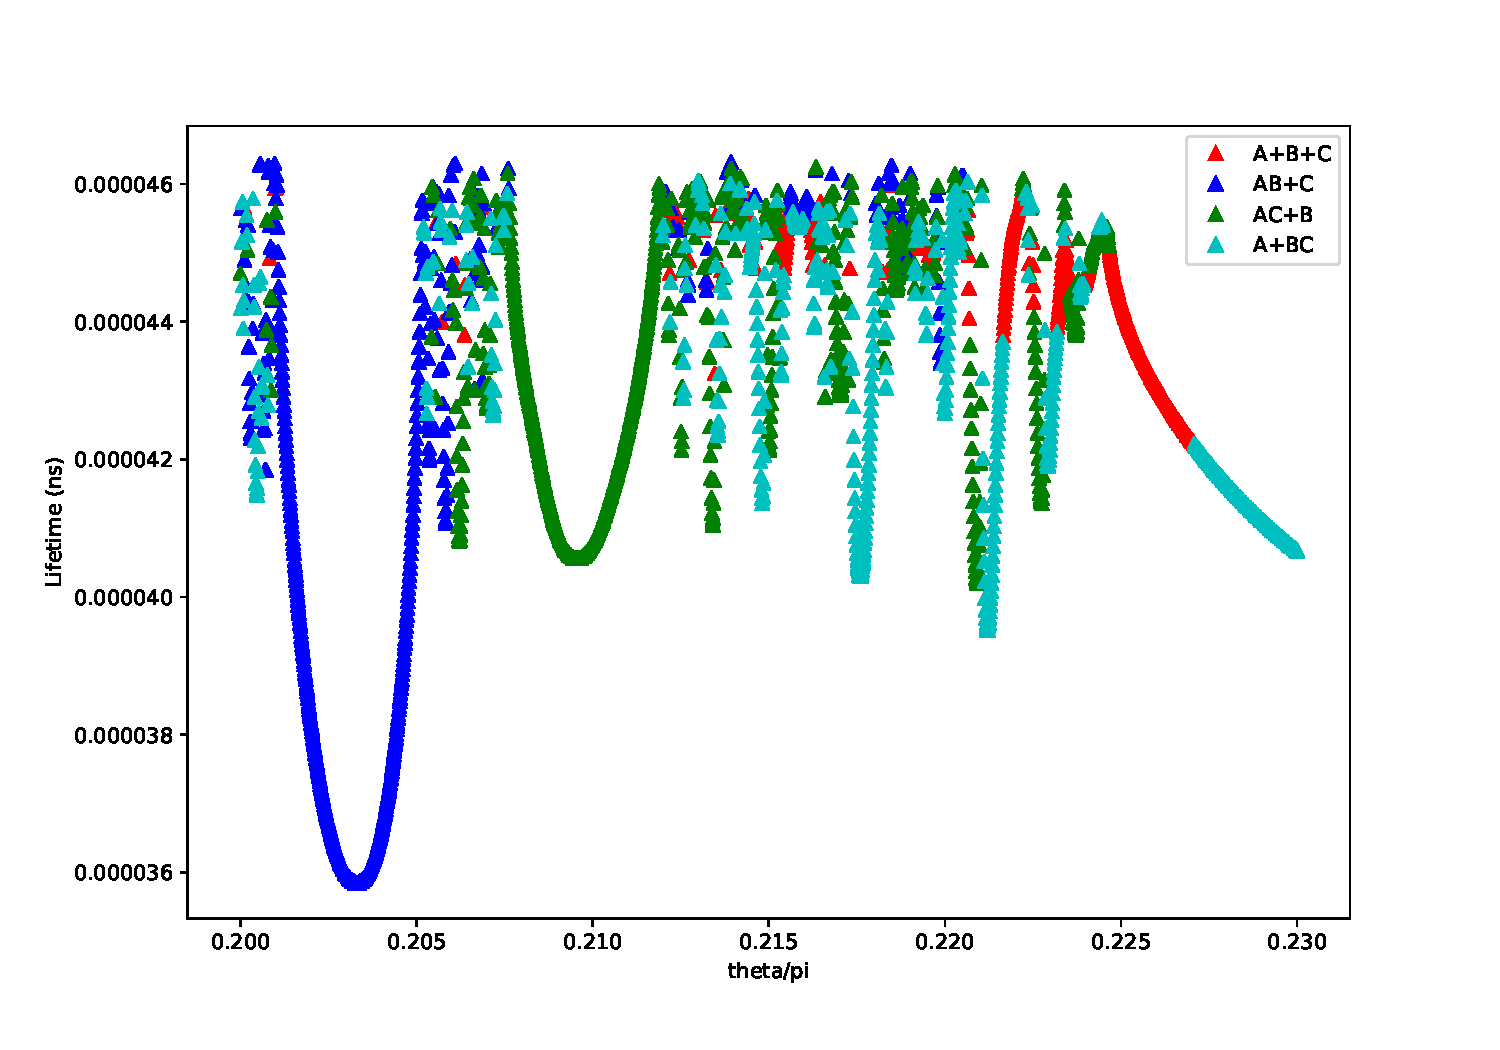
\includegraphics[clip,width=1.1\columnwidth]{fractal_zoomed.pdf}%
}
\label{fig:chaos}
\caption{Lifetime and ending ``basin"  for $\mathrm{Li} + \mathrm{Li_2}$ at $T = 350~\mathrm{K}$ as a function of the initial orietnation angle of the dimer $\theta$. The lower panel is a zoomed in version of the upper one, illustrating the scale invariance property of the system.
}
\end{figure}

The fractal dimension~\cite{mandelbrot1967} characterizes how much the fractal pattern changes as one changes the scale of the system, so it is a way to quantify the scale invariance and, as we shall see, also the moment of onset of chaos. We following the so-called ``uncertainty algorithm" to define the fractal dimension, $d$~\cite{mcdonald1985}. As already discussed, we classify trajectories by the "basin" they end up in. A trajectory is further classified as unstable under perturbation of initial conditions if by changing the initial variables by a value $\delta$ the outcome ends being part of a different basin than the original one. As such, we compute a large number of pairs of trajectories, where the pairs differ only in that $\theta$ is changed by an amount $\delta$. We then compute the fraction of unstable trajectories, which is observed to be characterized by

\begin{equation}
f(\delta, E_{\mathrm{col}}) \propto \delta^{\alpha(E_{\mathrm{col}})},
\end{equation}
where $E_{\mathrm{col}}$ is the collision energy, $\delta$ is the perturbation we apply (to the angle $\theta$), and $\alpha$ is the uncertainty exponent that we fit~\cite{mcdonald1985}. Figure~\ref{fig:unc} illustrates some of the results for a wide range of temperatures, from which we can conclude that at high collision energies the trajectories are essentially stable under perturbation, with the unstable fraction decreasing as $\delta$ gets smaller, while for lower collision energies the unstable fraction is essentially independent of $\delta$, meaning that there is no correlation between the outcomes of trajectories that are arbitrarily closely ``neighboring" in the phase space of initial conditions. We can again interpret this as saying that during such a collision the energy is constantly redistributed between the constituent atoms randomly, destroying any correlation with the initial conditions.

\begin{figure}[ht]
\begin{center}
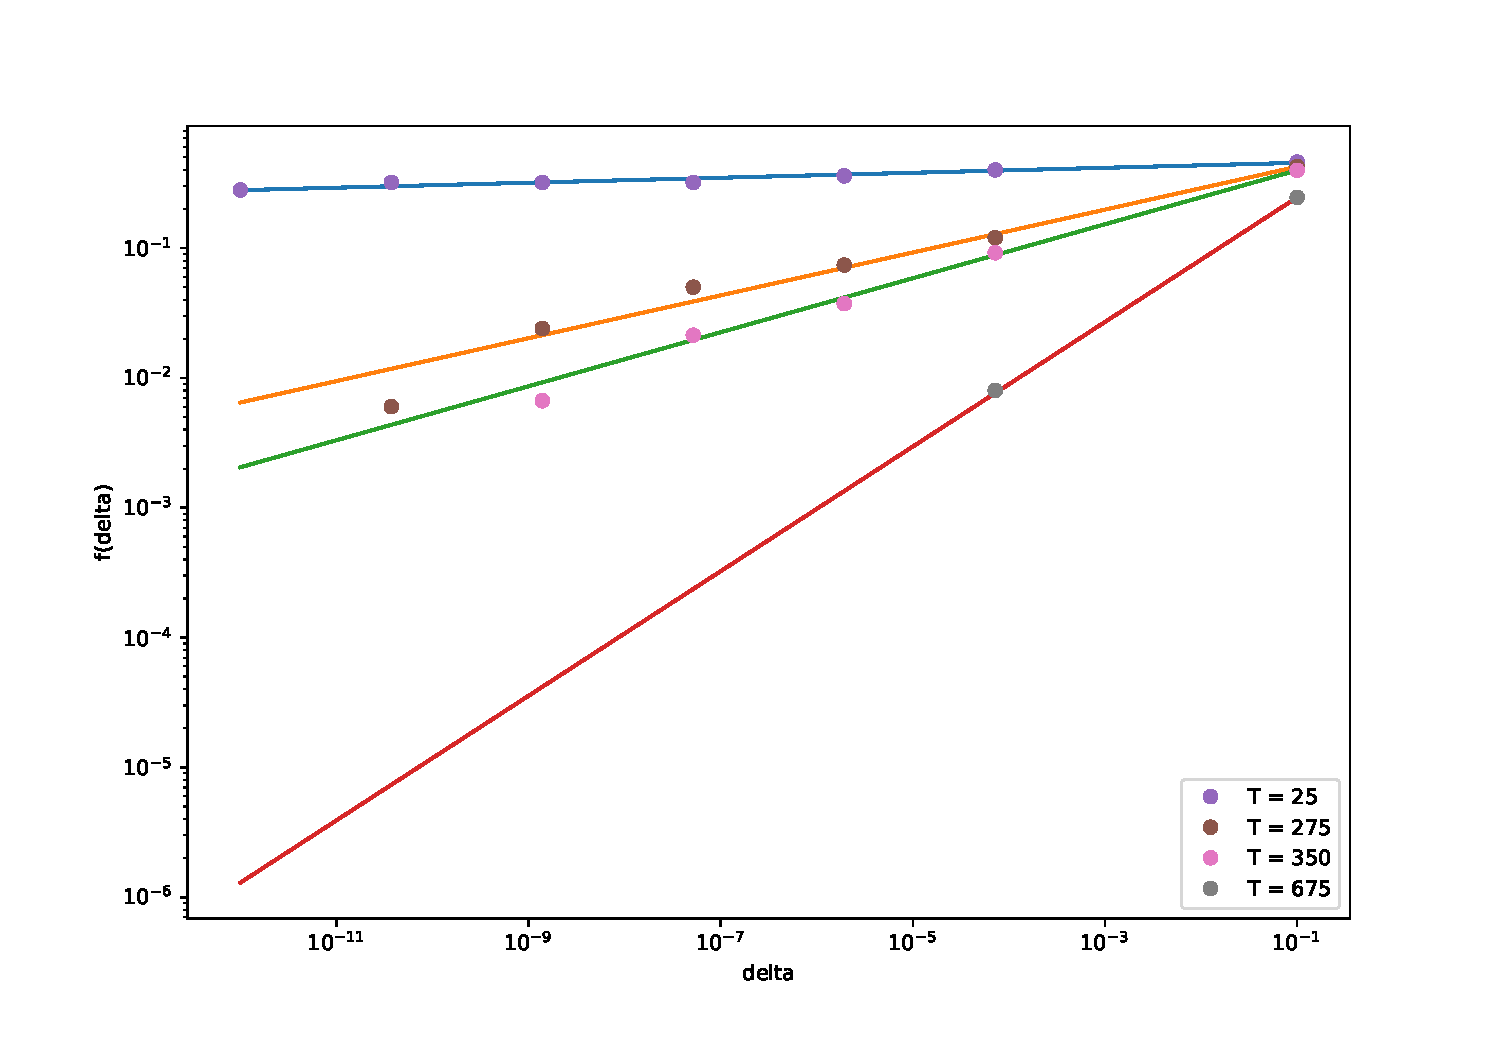
\includegraphics[width=1.125\linewidth]{uncertainty.pdf}
\caption{The unstable fraction of trajectories, $f(\delta)$, as a function of the perturbation value $\delta$ for $\mathrm{Li} + \mathrm{Li_2}$. At $25$ K $\alpha$ is $0.02$, corresponding to trajectories that are completely sensitive to initial conditions' perturbations, while at $250$ K and $675$ K it is $0.2$ and $0.48$, respectively.}
\label{fig:unc}
\end{center}
\end{figure}

As in~\cite{bohn2014,mcdonald1985}, we can relate $\alpha$ to the fractal dimension through the relation $\alpha = D-d$, where in our case $D = 1$. This is because $\alpha$ is related to the boundary between different regions of stability in phase space: when $\alpha$ is near 0, the basin boundary essentially fills all of space and so every point in phase space leads to a different outcome; conversely, when $\alpha$ is near 1, the basins are well defined and orbits are less chaotic. Hence, by fitting determining $\alpha$ for each collision energy, we have a direct way to characterize the fractal dimension. This characterization is shown for the case of Li atoms in Fig.~\ref{fig:frac_dim}. As is seen there, the factal dimension is large for low collisions energies and falls off quickly around a few hundred K, indicated by the vertical line.


\begin{figure}[ht]
\begin{center}
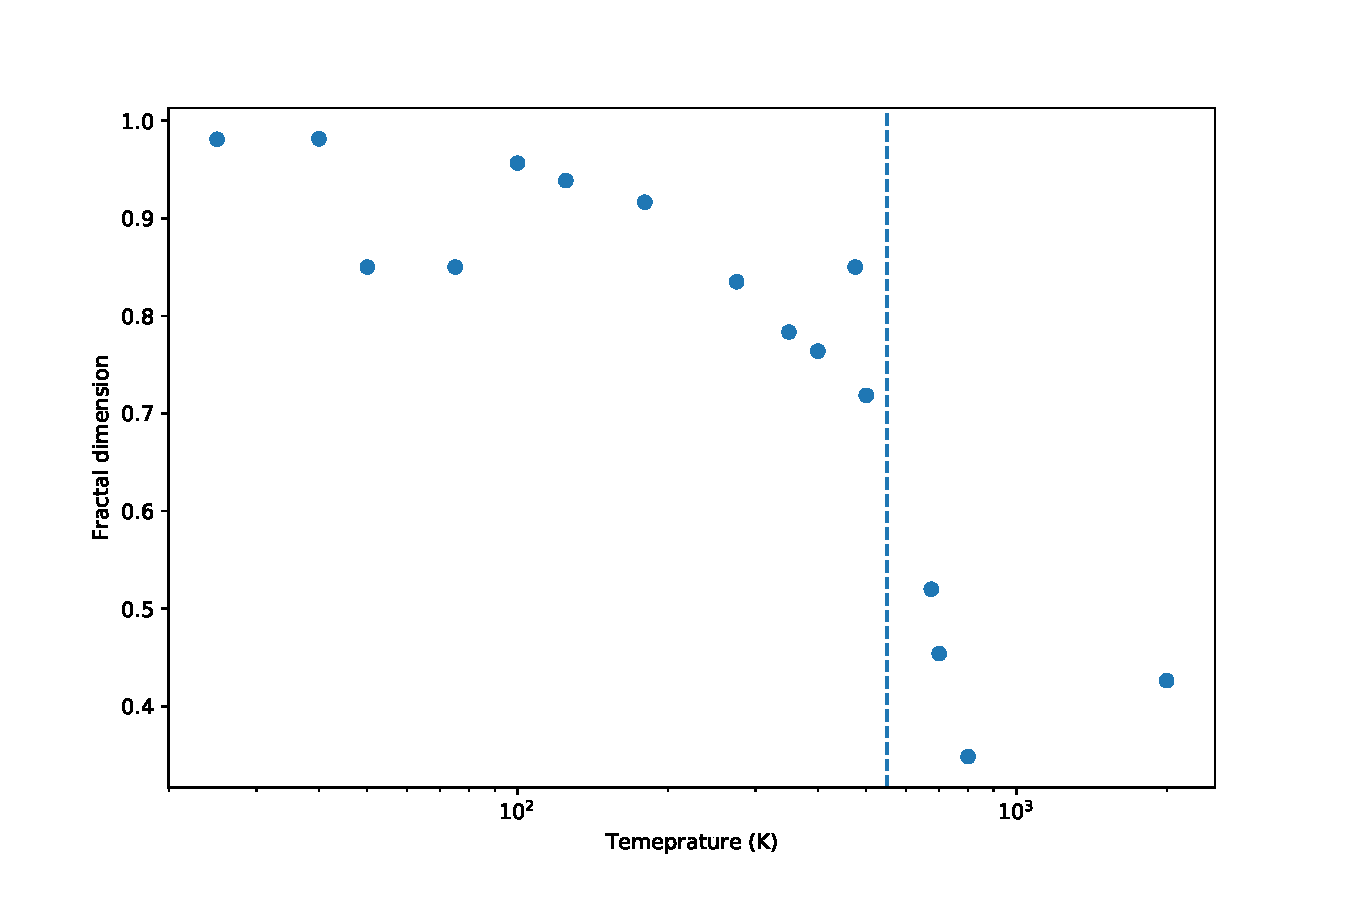
\includegraphics[width=1.125\linewidth]{fractal_dim.pdf}
\caption{Fractal dimension $d$ as a function of the collision energy of $\mathrm{Li} + \mathrm{Li_2}$. The vertical line marks the approximate energy at which chaotic behvior ensues.}
\label{fig:frac_dim}
\end{center}
\end{figure}

 
%\begin{figure}[ht]
%\begin{center}
%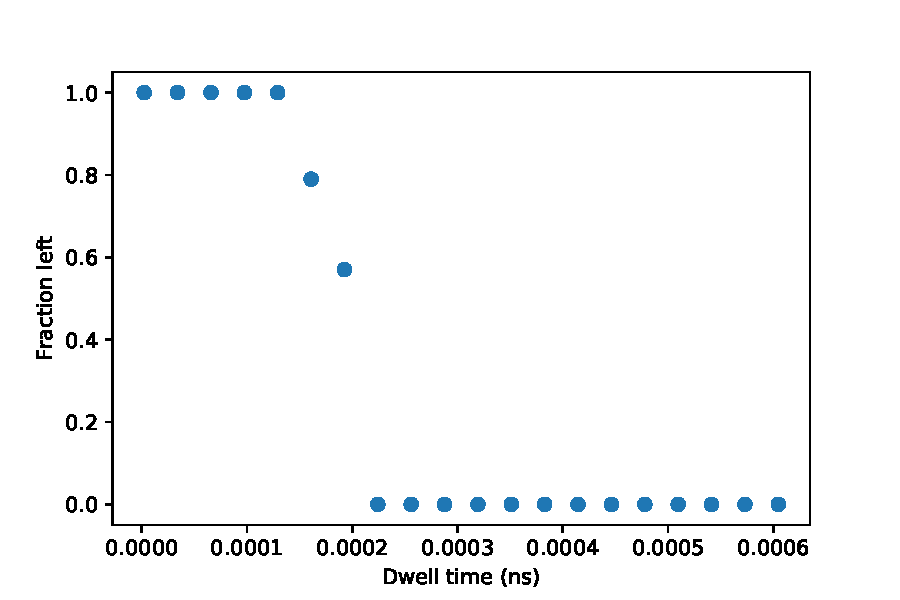
\includegraphics[width=1\linewidth]{fraction_left.pdf}
%\caption{}
%\label{fig:lifetime}
%\end{center}
%\end{figure}

\section{\label{sec:RRKM}Semi-classical Method: The RRKM Approximation}

\subsection{\label{sec:RRKM-overview} Overview}

On a semi-classical level, quantum scattering can be viewed as classical particles sampling the discrete quantum modes of the potential energy surface over the course of the encounter. Incoming particles collide and accelerate into the potential well, where the potential energy is converted into rotational and vibrational energies of the molecular complex. This is in contrast to the pure classical approach in the previous section, where states within the potential well are not quantized. 

In this picture, the Rice-Ramsperger-Kassel-Marcus (RRKM) theory~\cite{marcus1952-1,marcus1952-2} from chemistry suggests that the lifetime of a complex can be approximated as 
\al{
\tau_{dos} = \frac{2\pi\hbar\rho}{N_0}\label{eqn:rrkm}
}
where $\rho$ is the density of states (DOS) of the potential energy surface at the collision energy, and $N_0$ the number of open channels. Intuitively, this approximation assumes that over the course of the reaction, the collision complex samples all possible states over the potential energy surface. At high temperatures, $N_0$ may in general be large, and the lifetime is expected to be short. At ultracold temperatures however, the number of quantum states available to the collision is limited to a few, and we can even have $N_0=1$, giving experimentally observable lifetimes. Moreover, this can be compared to the classical approach, which serves as a foil for both theories.

While equation (\ref{eqn:rrkm}) is based on semi-classical grounds, the DOS of the energy spectrum must be found through quantum mechanical means. This involves solving for the bound states of the single channel Schrodinger equation. To this end, we utilize the mapped Fourier grid Hamiltonian (FGH) method \cite{clay1989,fattal1996}, which is well-suited for finding bound states of molecular potentials.


\subsection{\label{sec:FGH}Mapped Fourier grid Hamiltonian method}

\subsubsection{\label{sec:FGH-background}Background}

The single channel Shcrodinger equation we wish to solve is given by
\al{
\hat{H}\ket{\psi} = E\ket{\psi}
}
where the Hamiltonian $\hat{H}$ as an operator can in general consist of the kinetic energy part $\hat{T}$ and a potential energy part $V(\hat{x})$ independent of momentum
\al{
H = \hat{T} + V(\hat{x}) = \frac{\hat{p}^2}{2m} + V(\hat{x})
}
In particular, we are interested in bound states of this system, which are given by the condition $E<0$.

The potential energy is diagonal in the coordinate basis, whereas the kinetic energy is diagonal in momentum space basis, i.e.
\al{
\bracket{x}{V}{x'} &&= V(x)\delta(x-x')\\
\bracket{k}{T}{k'} &&= \frac{\hbar^2 k^2}{2m}\delta(k-k')
}
where we have defined
\al{
\hat{x}\ket{x} = x\ket{x},\ \hat{p}\ket{k}=\hbar k\ket{k}
}
The main idea of the FGH method is to utilize the fact that position space and momentum space representations of a wavefunction are Fourier transforms of each other. This means that to find the matrix elements of the Hamiltonian, we can Fourier transform from position space into momentum space to evaluate the kinetic energy operator where it is diagonal, then inverse Fourier transform back into position space.

\subsubsection{\label{sec:FGH-theory}Theory}

To begin with, we write out the matrix elements of the Hamiltonian exactly in the position basis representation.
\al{
\bracket{x}{H}{x'} &&= \bracket{x}{V}{x'} + \bracket{x}{T}{x'} \nonumber \\ 
&&=\int_{-\infty}^\infty\braket{x}{k}T\braket{k}{x'}dk + V(x)\delta(x-x')\nonumber 
\\ &&= \frac{1}{2\pi}\int_{-\infty}^\infty e^{ikx}T_ke^{-ikx'}dk + V(x)\delta(x-x')\label{eqn:fgh-continuous} \\
}
where we have defined 
\al{
T_k=\frac{\hbar^2k^2}{2m}
} 
and used the relation
\al{
\braket{k}{x}=\frac{1}{\sqrt{2\pi}}e^{-ikx}
}

In the FGH method, we discretize position space in the range $[0,x_{max}]$ by an even grid of $N$ points, so that the spacing of each step is $\Delta x$ and denote
\al{
x_i=i\Delta x.
}
As a result, momentum space is discretized correspondingly in a reciprocal manner, where the range and spacing of the momentum space grid is determined by those in position space. In particular, the grid is limited to the range $[-k_{max},k_{max}]$ where $k_{max} = \frac{\pi}{\Delta x}$ and is discretized into $N$ points with 
\al{
\Delta x \Delta k = \frac{2\pi}{N}
}
As for the position space grid, we denote
\al{
k_i = i\Delta k
}
With such a discretization, the potential and kinetic potential parts in equation (\ref{eqn:fgh-continuous}) become
\al{
\bracket{x_i}{V}{x_j} && = V(x_i)\delta_{ij} \\
\bracket{x_i}{T}{x_j} &&= \frac{1}{2\pi}\sum_{l=-N/2}^{N/2}e^{ik_lx_i}\cdot T_{k_l}\cdot e^{-ik_lx_j}\Delta k \nonumber \\
&& = \frac{1}{2\pi}\frac{1}{N}\sum_{l=-N/2}^{N/2}e^{i2\pi l i/N}\cdot T_{k_l}\cdot e^{-i2\pi lj/N}
}
Putting these together gives the Hamiltonian in the discretized coordinate space grid
\al{
H_{ij} &&= \bracket{x_i}{H}{x_j} \nonumber \\
&& = \frac{1}{2\pi N} \sum_{l=-N/2}^{N/2}e^{il2\pi i}\cdot T_l \cdot e^{-il2\pi j}+V(x_i)\delta_{ij} \label{eqn:fgh-discrete}
}

This equation is the crux of the FGH method. It can also be put in the form of a Fourier transform then inverse Fourier transform. In particular, if we let
\al{
\phi_n =(0,&&..,0,1,0,...,0)^T\\
&& \text{n-th index}
}
be a basis vector in position space, then the n-th column of the Hamiltonian can be expressed as
\al{
H_{in} = [(\mathcal{F}^{-1}T\mathcal{F}+V)\phi_n]_i
}
where $\mathcal{F}$ is the Fourier transform operator and $T$ is the diagonal operator $\diag{T_{k_l}}$. This equation is equivalent to equation (\ref{eqn:fgh-discrete}), but explicitly shows the use of the Fourier transform into momentum space. One of the advantages of this method is that the Fourier transform can be completed efficiently by means of the discrete fast Fourier transform (DFFT).

In principle, from here we may diagonalize this Hamiltonian to obtain the energy values and wavefunctions we desire. The FGH method presented as is however, can only be implemented on an evenly spaced grid. This can be problematic with many potentials of interest in atomic and molecular physics, where potentials consist of a small potential well region that then asymptotes to zero at large distances. In the potential well, the wavefunction oscillates rapidly, whereas it decays exponentially in the classically forbidden region. Since rapid oscillations correspond to large momentum, and large momentum range requires small grid spacing in position space, one would optimally hope to have a denser grid in the potential well than in the classically forbidden region.

This can be achieved by taking a nonlinear mapping from original coordinates $(x)$ to a new set of coordinates $(Q)$. The representation of the kinetic energy term in position basis is given as 
\al{
T = -\frac{\hbar^2}{2m}\left(J^{-1}(Q)\frac{\partial}{\partial Q}\right)^2
}
where $J=\frac{\partial x}{\partial Q}$. This term can then be found from position space by taking two Fourier transform and inverse Fourier transform pairs in sequence. 
\al{
H_{in} = [(J^{-1}\mathcal{F}^{-1}\sqrt{T}\mathcal{F}J^{-1}\mathcal{F}^{-1}\sqrt{T}\mathcal{F}+V)\phi_n]_i
}
where we have used $\sqrt{T}$ to denote $\diag{\sqrt{T_{k_l}}}$. This gives the mapped FGH method, which typically performs much better in convergence compared to its even grid counterpart.

The mapping 
\al{
x = Q-A\arctan(\beta Q)
}
where $A,\beta$ are parameters that can be optimized, turns out to have nice properties for the current problem of interest~\cite{fattel1996}. This is plotted in Fig.~\ref{fig:mapping}, where we see that the grid is denser at small distances and gradually sparsens at large distances.

\begin{figure}
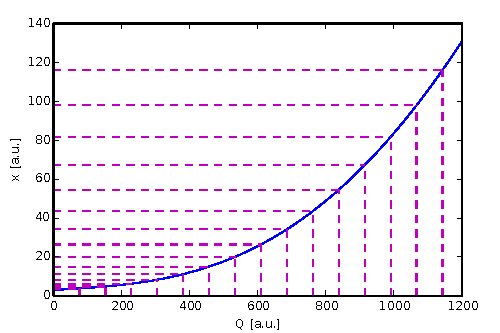
\includegraphics{figures/mapping}
\caption{\label{fig:mapping}Mapping of coordinates $x = Q-A\arctan(\beta Q)$, where $A=2000, \beta = 1/2020$}. The grid gives a denser sampling for small distances than at large distances as desired.
\end{figure}

\subsection{Density of states and lifetime}

To find the density of states relevant for applying RRKM theory, we need to consider the bound states that arise from both the long range atom+dimer collision and the short range atom+atom interactions that form dimers. In both these cases, the potential in the radial part of Schrodinger's equation can be approximated as a Lennard-Jones potential of the form
\al{
V^{(L)}_{LJ}(R) = \frac{C_{12}}{R^{12}} - \frac{C_6}{R^6} + \frac{L(L+1)}{2\mu R^2}
}
where $L$ denotes the partial wave number (more details in Sec.~\ref{sec:QuantumTraj}).

For the short range dimer states, the $C_{6,A_2}$ and $D_{e,A_2}$ values are taken as in Table~\ref{table:coeffs}. Each of the ro-vibrational bound states of this potential gives an atom+dimer collision channel. We label the energy for each of these ro-vibrational states as $E_{v,n}$, where $v,n$ denote the vibrational and rotational number respectively. An example of this is given in Fig.~\ref{fig:li_dimer_wavefunctions}.

\begin{figure}
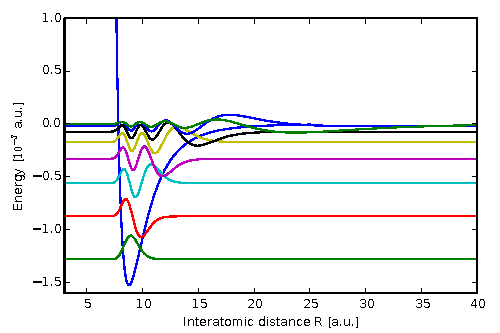
\includegraphics{figures/li_li_n0_wavefunctions}
\caption{\label{fig:li_dimer_wavefunctions}Wavefunctions and corresponding energy levels of Li+Li system with angular momentum number $n=0$.}
\end{figure}

To find the long range bound states, we assume that $C_{6,A_2+A} = 2C_{6,A_2}$ and $D_{e,A_2+A}=2D_{e+A_2}$. The bound states of this long range interaction gives another series of energy levels $E_{L,\alpha}$. As above, $L,\alpha$ label the angular momentum and vibrational numbers respectively. 

Now, each asymptotic ro-vibrational channel gives an offset in the collision threshold as $E_{L,\alpha,v,n} = E_{L,\alpha}+E_{v,n}$. The aggregate series $E_{L,\alpha,v,n}$ constitutes the spectrum consisting of the bound states over the reaction potential surface.

We note that conservation of angular momentum requires that $\ve{J}=\ve{L}+\ve{n}$, so that relevant restrictions are placed on the values of $L,n$. In particular, for the case of S-wave collisions, $J=0$, so that $L=n$. Moreover, we need to account for any degeneracies arising from the magnetic quantum number. For instance, in the case the total magnetic quantum number $M=M_L+m_n=0$ vanishes, there is a degeneracy of $2L+1$ for each corresponding energy level.

\begin{figure}
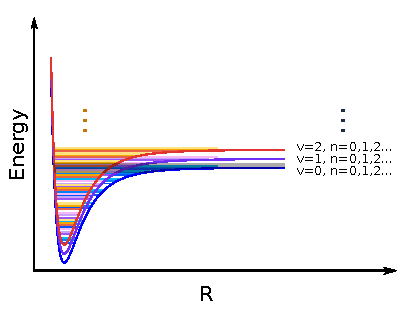
\includegraphics{figures/dos}
\caption{\label{fig:dos}Schematic of method to find DOS near ro-vibrational ground state threshold (not to scale). Each potential energy curve represents an atom+dimer interaction potential (blue, purple, orange series). Horizontal lines in each color series belong to the series $E_{\alpha}^L$ for a given $(v,n)$. The energy is offset by the atom+atom bound state energy. These combined give rise to the energy spectrum $E_\alpha^{(L,v,n)}$. We count the number of states in the gray shaded area to find an average DOS near the ro-vibrational collision threshold.}
\end{figure}


At ultracold temperatures, the incoming/outgoing channel is restricted to the rovibrational ground state $\nu = 0, n = 0$. To find the DOS around this energy level, we count the average number of states within a given energy interval.

Fig.~\ref{fig:dos} summarizes the process of finding the energy spectrum. In our implementation, we take $J=0$ (corresponding to vanishing impact parameter $b=0$ classically) and $M=M_L+m_n=0$. We list our results of the DOS and corresponding complex lifetime as computed from Eq.~\ref{eqn:rrkm} in Table~\ref{tab:dos}. We find that the results agree with those obtained from the classical trajectories to within a factor of 2. This is remarkable, as it suggests that the classical approach is sufficient for certain observables of interest. 

\begin{table}[b]
\caption{\label{tab:dos}Density of states}
\begin{ruledtabular}
\begin{tabular}{cccc}
 Atom species & DOS [$\text{mK}^{-1}$] & $\tau_{dos}$ [ns] & $\tau_\text{classical}$ [ns]\\ 
\hline
Li & 0.06 & 2.8 & dd \\
K & 2.52 & 120 & dd \\
Cs & 32.15 & 1542 & dd
\end{tabular}
\end{ruledtabular}
\end{table}





\section{\label{sec:QuantumTraj}Quantum Mechanical Method}
Because, ultimately, quantum mechanics rules the day\footnote{Barring a \textit{truly} remarkable discovery in the coming days.}, the ``gold standard" solution to any scattering problem is surely quantum mechanical in nature. What this entails is solving the Schrodinger equation for the two particles moving under the influence of their mutual interaction and any external electromagnetic fields. As long as these external fields have no time variation, the solution to the time-\textit{independent} Schrodinger equation will be sufficient to extract physically meaningful observables. Here, we briefly describe the necessary quantum mechanical formalism before delving into numerical methods.

\subsection{\label{sec:QuantumFormalism} Formulating the Quantum Problem}
We consider two particles, $A$ and $B$, whose \textit{internal} quantum states are described by the Hamiltonians $H_A$ and $H_B$, respectively. In quantum mechanics, the Hamiltonian is an operator (matrix) which represents the total energy of the system. In particular, we will assume the Hamiltonians give rise to eigenstates (eigenvectors) and eigenvalues denoted by $H_A \lvert \alpha \rangle = E_\alpha \lvert \alpha \rangle$, and similarly for particle $B$. The eigenstates $\lvert \alpha \rangle$ and $\lvert \beta \rangle$ represent a complete specification of the state of each particle: for instance, $\alpha$ is a composite label which describes the electronic state of the particle including the principal quantum number (the gross ``energy level" the molecule is in), the electronic angular momentum (due to an electron's orbit around the nucleus), the electron's spin state (which may be ``up" or ``down"), and any coupling between these angular momenta called ``fine" and ``hyperfine" structure--- which simply give rise to small energy splittings depending on the relative orientations of the electron's orbital rotation and the direction of it, or the nucleus', intrinsic spin angular momentum. The \textit{total} Hamiltonian of this two-particle system can be written as,

\begin{equation}
H_\text{tot} = -\frac{\hbar^2}{2m_A} \nabla_A^2 -\frac{\hbar^2}{2m_B}\nabla_B^2 + U(\mathbf{r}_A,\mathbf{r}_B) + H_A + H_B,
\end{equation}

\noindent where the first two terms represent the kinetic energies of each particle, $U$ represents the interaction potential energy between the two particles, and the last two terms are the internal Hamiltonians described above. It is assumed that $U$ vanishes when the separation between the two particles becomes very large, as their interactions should vanish as they are increasingly isolated. 

It is a standard exercise~\cite{ColdChemBook,Krems2017} to convert from laboratory-fixed coordinates to so-called ``relative coordinates" where $\mathbf{r}$ is the relative displacement between the particles' centers of mass. Then, the Hamiltonian is written as,

\begin{equation}
H_\text{tot} = -\frac{\hbar^2}{2\mu} \nabla_r^2 + U(\mathbf{r}) + H_A + H_B,
\label{eq:SchrodFinal}
\end{equation}

\noindent where the first term now describes the \textit{relative} kinetic energy between the particles ($\mu$ is their reduced mass) and the interaction potential now depends only on their relative separation. The center-of-mass motion is ignored because, in nearly every case of interest, it contributes only overall offsets to energies and has no observable consequence beyond this. (Recall that only energy \textit{differences} are physically relevant anyway.) We can express the kinetic energy operator in spherical polar coordinates as

\begin{equation}
-\frac{\hbar^2}{2\mu} \nabla_r^2 = -\frac{\hbar^2}{2\mu} \frac{1}{r^2} \frac{\partial}{\partial r} r^2 \frac{\partial}{\partial r} + \frac{\hbar^2 \mathbf{L}^2(\theta,\phi)}{2\mu r^2}
\end{equation}

\noindent where $\mathbf{L}^2(\theta,\phi)$ is the angular momentum operator describing the rotations of $\mathbf{r}$ in space, whose eigenstates are well-known as the spherical harmonics: $\mathbf{L}^2(\theta,\phi) \lvert \ell, m_\ell \rangle = \ell(\ell+1) \lvert \ell,m_\ell \rangle$. 

The goal of a quantum scattering calculation is, therefore, simply to solve the Schrodinger equation $H_\text{tot} \lvert \Psi \rangle = E \lvert \Psi \rangle$ assuming a specific energy and specific internal states $\lvert \alpha \rangle$ and $\lvert \beta \rangle$ for the incoming particles. By the tenants of quantum mechanics, the scattering wavefunction $\lvert \Psi \rangle$ can then be used to obtain any physically measurable properties of the collision. It is typical to expand the state $\lvert \Psi \rangle$ as a sum over all the possible incoming internal states of each particles, and over all possible incoming angular momentum states: 

\begin{equation}
\lvert \Psi \rangle =  \sum_{\alpha,\beta,\ell,m_\ell} \frac{1}{r} F_{\alpha \beta \ell m_\ell}(r) \lvert \alpha \beta \ell m_\ell \rangle
\label{eq:BasisExpansion}
\end{equation}

\noindent where $\lvert \alpha \beta \ell m_\ell \rangle = \lvert \alpha \rangle \otimes \lvert \beta \rangle \otimes \lvert \ell \rangle \otimes \lvert m_\ell \rangle$ represents a tensor product of the basis states of each particle's internal state, and the relative angular momentum. The complete set of quantum numbers to describe an incoming internal and angular momentum state of a collision complex is often called a \textit{channel}. $F_{\alpha \beta \ell m_\ell}(r)$ is the amplitude to be in each basis state. The sum extends over all possible internal states, all $\ell = 0, 1, ..., \infty$, and $m_\ell = -\ell, ..., \ell$. In practice, the expansion over basis states is usually truncated to include only the internal states which are coupled by the interaction $U$ and only enough angular momentum states (called ``partial waves") to achieve convergence. This will be discussed in the calculations carried out detail below. 

Plugging $\lvert \Psi \rangle$, Eq.~\ref{eq:BasisExpansion}, into the Schrodinger equation, Eq.~\ref{eq:SchrodFinal}, and recognizing that $r^{-2} \frac{\partial}{\partial r} r^2 \frac{\partial}{\partial r} \frac{F(r)}{r} = r^{-1} \frac{\partial^2}{\partial r^2} F(r)$, we obtain:

\begin{widetext}
\[
\sum_{\alpha,\beta,\ell,m_\ell} \left(\frac{d^2}{dr^2} - \frac{\ell(\ell+1)}{r^2} + \frac{2 \mu}{\hbar^2}(E-E_A-E_B) \right) F_{\alpha \beta \ell m_\ell}(r)  \lvert \alpha \beta \ell m_\ell \rangle = \frac{2 \mu}{\hbar^2} \sum_{\alpha,\beta,\ell,m_\ell} U(r) F_{\alpha \beta \ell m_\ell}(r)  \lvert \alpha \beta \ell m_\ell \rangle 
\]
\end{widetext}

\noindent Now, projecting out a single quantum state by left-multiplying both sides of the equation by $\langle \alpha^\prime \beta^\prime \ell^\prime m_\ell^\prime \rvert$, we obtain (since the eigenstates of a Hermitian operator like the Hamiltonian must be orthogonal) the \textit{coupled-channel equations}:
\begin{widetext}
\[
 \left(\frac{d^2}{dr^2} - \frac{\ell(\ell+1)}{r^2} + k_{\alpha \beta}^2 \right) F_{\alpha \beta \ell m_\ell}(r) = \frac{2 \mu}{\hbar^2} \sum_{\alpha^\prime,\beta^\prime,\ell^\prime,m_\ell^\prime} \langle \alpha \beta \ell m_\ell \rvert U(r)   \lvert \alpha^\prime,\beta^\prime,\ell^\prime,m_\ell^\prime \rangle F_{\alpha^\prime,\beta^\prime,\ell^\prime,m_\ell^\prime}(r),
 \]
\end{widetext}

\noindent where $k_{\alpha \beta}^2 = \frac{2\mu}{\hbar^2}(E-E_A-E_B)$ and, for convenience, the primed and unprimed labels have been swapped. We have thus obtained a set of coupled, second-order differential equations for the coefficients $F_{\alpha \beta \ell m_\ell}$ which expand the state over the various collision channel. It is clear the the interaction potential may \textit{couple} the various channels, and thereby change the states of one or either of the particles as they exit the collision. Our problem is therefore to determine the coefficients $F_{\alpha \beta \ell m_\ell}$, which then let us describe the collision wavefunction in the basis of internal states and angular momentum states (which are all assumed to be known, at least numerically). 

One question remains before we can fully solve the coupled-channel equations: what are the boundary conditions? Physical reasoning gives these easily. First, as $r \rightarrow 0$, there must exist a repulsive barrier preventing the nuclei from overlapping. Hence, $F_{\alpha \beta \ell m_\ell}(r\rightarrow 0) = 0$ for all possible quantum numbers. Second, as $r \rightarrow \infty$, the wavefunctions must approach well-known analytical solutions to the scattering problem. It is a standard (though tedious) problem in introductory quantum mechanics courses to determine these~\cite{Krems2017,ColdChemBook}, so we omit the proof here and simply state the result: At long range, the scattering wavefunctions are described as linear combinations of spherical Bessel functions, $j_\ell$ and $y_\ell$. The method of matching the two boundary conditions in the numerical solution will be outlined below.

With the solution wavefunction in hand, we can derive physically meaningful observables. These come in the form of an ``S-matrix" which summarizes the probability for states to scatter from one to another. The S-matrix is a unitary operator, whose off-diagonal components describe the probability of a transition from one basis state to another~\cite{Krems2017,ColdMolsBook,ColdChemBook}. We describe how the S-matrix is computed numerically below, where it is the main observable our calculations predict.

\subsection{\label{sec:QuantumMethod} Numerical Methods for the Quantum Problem}
We now describe in detail popular numerical methods for solving the coupled-channel quantum scattering problem. We consider first the simple case of a single-channel problem, in which we merely need to solve the scalar Schrodinger equation $-\frac{\hbar^2}{2m} \frac{d^2}{dx^2} \psi(x) + V(x) \psi(x) = E \psi(x)$. Let us now derive a numerical method to solve this equation. 

\subsubsection{Single-Channel Case}

First, rewrite the Schrodinger equation as $\psi^{\prime\prime}(x) = k(x) \psi(x)$ where $k^2(x) = \frac{2m}{\hbar^2} (E-V(x))$. Define an equally spaced grid of points, $x_0, x_1,..., x_N$ with spacing $h$. Taylor expanding $\psi(x)$ to 5th order and evaluating at grid points $n+1$ and $n-1$ and taking the difference between these we find:

%\begin{eqnarray*}
%\psi_{n+1} &=& \psi_n + h \psi_n^\prime + \frac{h^2}{2!} \psi^{\prime\prime}_n + \frac{h^3}{3!} \psi^{\prime\prime\prime}_n +  \frac{h^4}{4!} \psi^{(4)}_n + \frac{h^5}{5!} \psi^{(5)}_n + \mathcal{O}(h^6) \\
%\psi_{n-1} &=& \psi_n - h \psi_n^\prime + \frac{h^2}{2!} \psi^{\prime\prime}_n - \frac{h^3}{3!} \psi^{\prime\prime\prime}_n +  \frac{h^4}{4!} \psi^{(4)}_n - \frac{h^5}{5!} \psi^{(5)}_n + \mathcal{O}(h^6)
%\end{eqnarray*}
%
%\noindent Using the fact that odd-ordered terms experience a change of sign between grid points $n+1$ and $n-1$, we can sum these two equations to obtain:

\begin{equation}
\psi_{n+1} - 2 \psi_n + \psi_{n-1} = h^2 \psi_n^{\prime\prime} + \frac{h^4}{12} \psi^{(4)}_n + \mathcal{O}(h^6)
\label{eq:Schrod1}
\end{equation}

\noindent We can take two more derivatives of the original equation  $\psi^{\prime\prime}(x) = k(x) \psi(x)$ to eliminate the fourth-derivative term here, using the exact same Taylor expansion logic to end up at the discrete formula

\begin{equation}
h^2 \psi^{(4)}_n = k^2_{n+1} \psi_{n+1} + 2 k^2_n \psi_n - k^2_{n-1} \psi_{n-1} + \mathcal{O}(h^4), 
\end{equation} 

\noindent whence, combining with Eq.~\ref{eq:Schrod1},

\begin{eqnarray*}
\psi_{n+1}-2\psi_n+\psi_{n-1} =& h^2k^2_n \psi_n + \frac{h^2}{12 } ( k^2_{n+1}\psi_{n+1} - \\ &2 k^2_n \psi_n + k^2_{n-1} \psi_{n-1} ) + \mathcal{O}(h^6)
\end{eqnarray*}

\noindent Note that this method is therefore fourth-order accurate. We can also rewrite it in a canonical form as a three-term recurrence relation:

\begin{eqnarray*}
\left( 1 - \frac{h^2}{12} k_{n+1}^2 \right)  \psi_{n+1} =& \left(2-\frac{10 h^2}{12}k_n^2 \right) \psi_n - \\ &\left( 1 + \frac{h^2}{12}k_{n-1}^2 \right) \psi_{n-1}
\end{eqnarray*}

\subsubsection{Multi-channel case}
Now let us return to the coupled-channel problem. Recall that we seek to solve $\left( \mathbb{I} \frac{d^2}{dr^2} + \mathbf{W}(r) \right) \mathbf{F}(r) = \mathbf{0}$, with $\mathbf{W}(r)$ defined as above\footnote{Here we have set $\hbar = 1$, to begin working in \textit{atomic units}.}. Again, define a grid of $N+1$ points uniformly spaced by $h$ between $r_0$ and $r_N$. The boundary condition at $r_0$ was identified above as $F(r_0) \equiv F_0 = \mathbf{0}$. We now propagate outward using the Numerov algorithm derived previously, generalized to matrix form (which is safely done due to diagonality of the kinetic energy term): 
\begin{equation}
\left(\mathbb{I}+\mathbf{T}_{n+1}\right) \mathbf{F}_{n+1} = \left(2\mathbb{I}+10\mathbf{T}_{n} \right)\mathbf{F}_n - \left(\mathbb{I}-\mathbf{T}_{n-1} \right) \mathbf{F}_{n-1}
\label{eq:MatrixNumerov}
\end{equation}

\noindent where $\mathbf{T}_n = -\frac{h^2}{12} 2 \mu \mathbf{W}(r_n)$. 

Johnson~\cite{JohnsonNumerov,Johnson73} made two important contributions to the development of this method. First, he noted that it is best to avoid numerical instabilities due to exponentially diverging solutions in the classically forbidden region\footnote{The region of space in which the total energy is less than the potential energy--- a region accessed only by quantum tunneling.} by using the following propagation method, called a ``renormalized Numerov" method. He defined a ``ratio matrix" $\mathbf{R}$ as $\mathbf{R}_{n+1} = \left( \mathbb{I} - T_{n+1}\right) \mathbf{F}_{n+1} \left((\mathbb{I}-\mathbf{T}_n)\mathbf{F}_n\right)^{-1}$. Note that if we define $\mathbf{U}_n = \left(2\mathbb{I}+10\mathbf{T}_n\right) \left(\mathbb{I}-\mathbf{T}_n\right)^{-1}$, then Eq.~\ref{eq:BasisExpansion} can be re-expressed as:
\begin{equation}
\mathbf{R}_{n+1} = \mathbf{U}_n - \mathbf{R}_n^{-1}
\end{equation}

\noindent which we will use as a recurrence relation for the matrix $\mathbf{R}$. Putting everything together, we can express the propagation routine as follows:

\begin{equation}
\mathbf{R}_{n+1} = -\mathbf{R}_n^{-1} + 12 \left(\mathbb{I} + \frac{h^2}{12} \mathbf{W}_n \right)^{-1} - 10\mathbb{I}
\end{equation}

\noindent Second, Johnson noted that by propagating the log-derivative matrix, defined as $\mathbf{Y} = \mathbf{F}^\prime \mathbf{F}^{-1}$, rather than $\mathbf{F}$ itself, an even simpler algorithm can be achieved. This is because in working with the log-derivative matrix, the second-order coupled-channels equations are turned into a set of first-order equations:

\begin{equation}
\frac{d \mathbf{Y}}{dr} + \mathbf{W}(r) + \mathbf{Y}^2(r) = 0
\label{eq:LogDerivEq}
\end{equation} 
\noindent as can be easily verified by plugging into the definition of the log-derivative to the coupled-channel equations. To solve this equation, Johnson derived an equivalent method and showed~\cite{Johnson73,JohnsonNumerov} that the following algorithm is also fourth-order accurate:

\begin{equation}
\mathbf{Y}_n = \left(\mathbb{I} + h \mathbf{Y}_{n-1}\right)^{-1} \mathbf{Y}_{n-1} - \frac{h}{3} w_n \mathbf{u}_n
\end{equation}

\noindent where $\mathbf{u}_n = \mathbf{W}(x_n), \,\, n = 0, 2,4,...N$ and $\mathbf{u}_n = \left( \mathbb{I} + \frac{h^2}{6} \mathbf{W}(x_n)\right)^{-1} \mathbf{W}(x_n),\,\,  n = 1, 3, 5, \cdots N-1$; and the weights are the same as in Simpson integration, i.e. $w_n = 1,\,\,  n = 0\text{ or } N$, $w_n = 4, \,\, n = 1, 3, 5, \cdots, N-1$, and $w_n = 2, \,\, n = 2, 4, 6, \cdots, N-2$. The log-derivative method can be derived following the same sorts of expansion arguments outlined above, and the order of accuracy is also derived in this way~\cite{ManJohnsonRederived,Johnson73,JohnsonNumerov,Friedman95}. We verify this property numerically below. Because this log-derivative method is the most popular among practitioners in the field of atomic and molecular collisions, we implement it in the calculations.

Finally, the log-derivative method obtains the S-matrix from the solution for $\mathbf{Y}$ by matching the large $r$ boundary conditions described above to the numerical solution. Matrices of Bessel functions of the first and second kind are defined via $\mathbf{J}_{ij} = \delta_{ij} k_j^{-1/2} \hat{j}_\ell(k_j x)$ and $\mathbf{N}_{ij} = \delta_{ij} k_j^{-1/2} \hat{n}_\ell(k_j x)$ where the functions with hats are Riccati-Bessel functions. An auxiliary matrix $\mathbf{K}$ is then defined by 

\begin{equation}
\mathbf{K} = -\left(\mathbf{Y}_N \mathbf{N}(x_N) - \mathbf{N}^\prime(x_N)\right)^{-1}  \left(\mathbf{Y}_N \mathbf{J}(x_N) - \mathbf{J}^\prime(x_N)\right)
\end{equation}

\noindent and then the S-matrix is obtained via 

\begin{equation}
\mathbf{S} = \left(\mathbb{I} + i \mathbf{K}\right)^{-1} \left( \mathbb{I} - i \mathbf{K} \right).
\end{equation}

\subsection{Numerical Implementation and Results}
Here, we summarize the results obtained from the log-derivative numerical integration scheme outlined above. The basis of the code for all results obtained below can be found in $\texttt{logderiv.py}$ and $\texttt{QuantumScattering.ipynb}$. We apply the method to two collisions of interest: a neutral atom - atomic ion collision, and a collision between a structureless molecule and a neutral atom with electronic spin. The theoretical results are compared to physical intuition for experimental results. 

Before this, we first check the expected convergence properties for the case of a constant potential energy matrix $\mathbf{U}$. This is the only case in which Eq.~\ref{eq:LogDerivEq} is analytically solvable, and its analytical solution is easily obtained by guess-and-check methods as $y(x) = V_0^{1/2} \cot(V_0^{1/2} x)$. We have run the log-derivative code for a variety of grid spacings, $h$, and at each step size have computed the relative error between the analytical and numerical solutions. The result is shown in Fig.~\ref{fig:ConvCheck}, and we indeed recover the expected fourth order scaling of the log-derivative method. 

\begin{figure}[b]
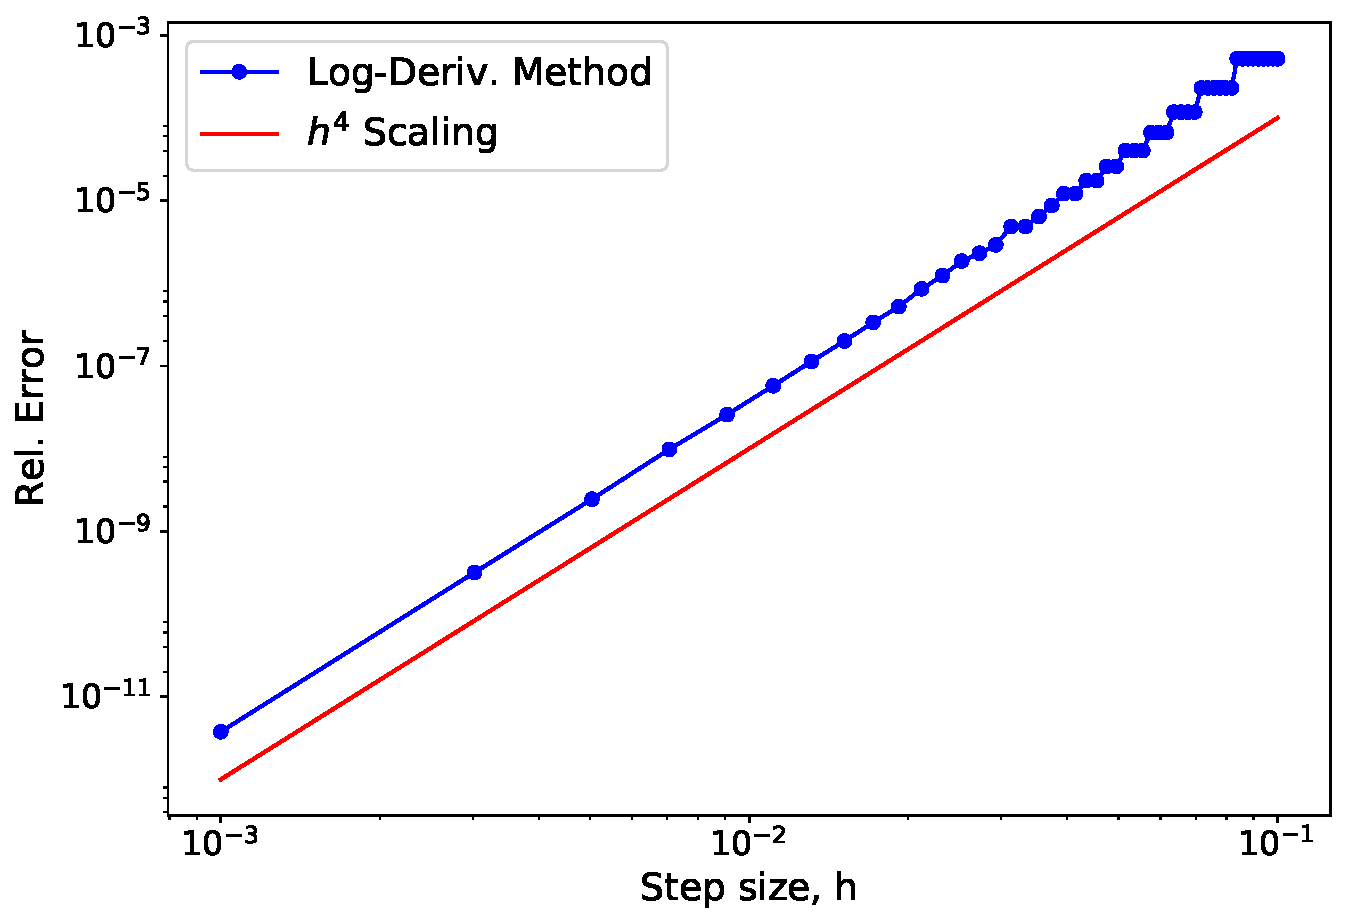
\includegraphics[width=1\columnwidth]{./Results/LogDerivErrorScaling}
\caption{Relative error in log-derivative integration as a function of step-size, $h$. The expected scaling is achieved.}
\label{fig:ConvCheck}
\end{figure}

%\subsubsection{Atom-Ion Collisions}
%
%We first consider a collision between a neutral Ne atom and an atomic He$^+$ ion. This collision is modeled as a two-channel collision, where the two channels represent two electronic states of the Ne atom: the collision may either leave the Ne atom in its ground state, or excite an outer-shell electron to an excited state about 17 eV higher in energy. The interaction matrix $\mathbf{U}$ therefore is $2\times 2$, with $U_{00} = a_1 r^{-1} e^{-r/a_2}$ representing the ground-state interaction, $U_{11} = (a_1 r^{-1} - a_3) e^{-r/a_2} + 16\text{ eV}$ representing the excited-state interaction, and $U_{01} = U_{10} = a_4 e^{-r/a_5}$ representing the mixing between the states. These potentials and constants are borrowed from~\cite{OlsonSmith71}, and the constants were determined there to be $a_1 = 21.1, a_2 = 0.678, a_3 = 12.1, a_4 = 0.17,$ and $a_5 = 0.667$, all in atomic units. We compute the collision properties at an energy of about 80 eV, which is an experimentally measurable regime. 

%\begin{figure}[tb]
%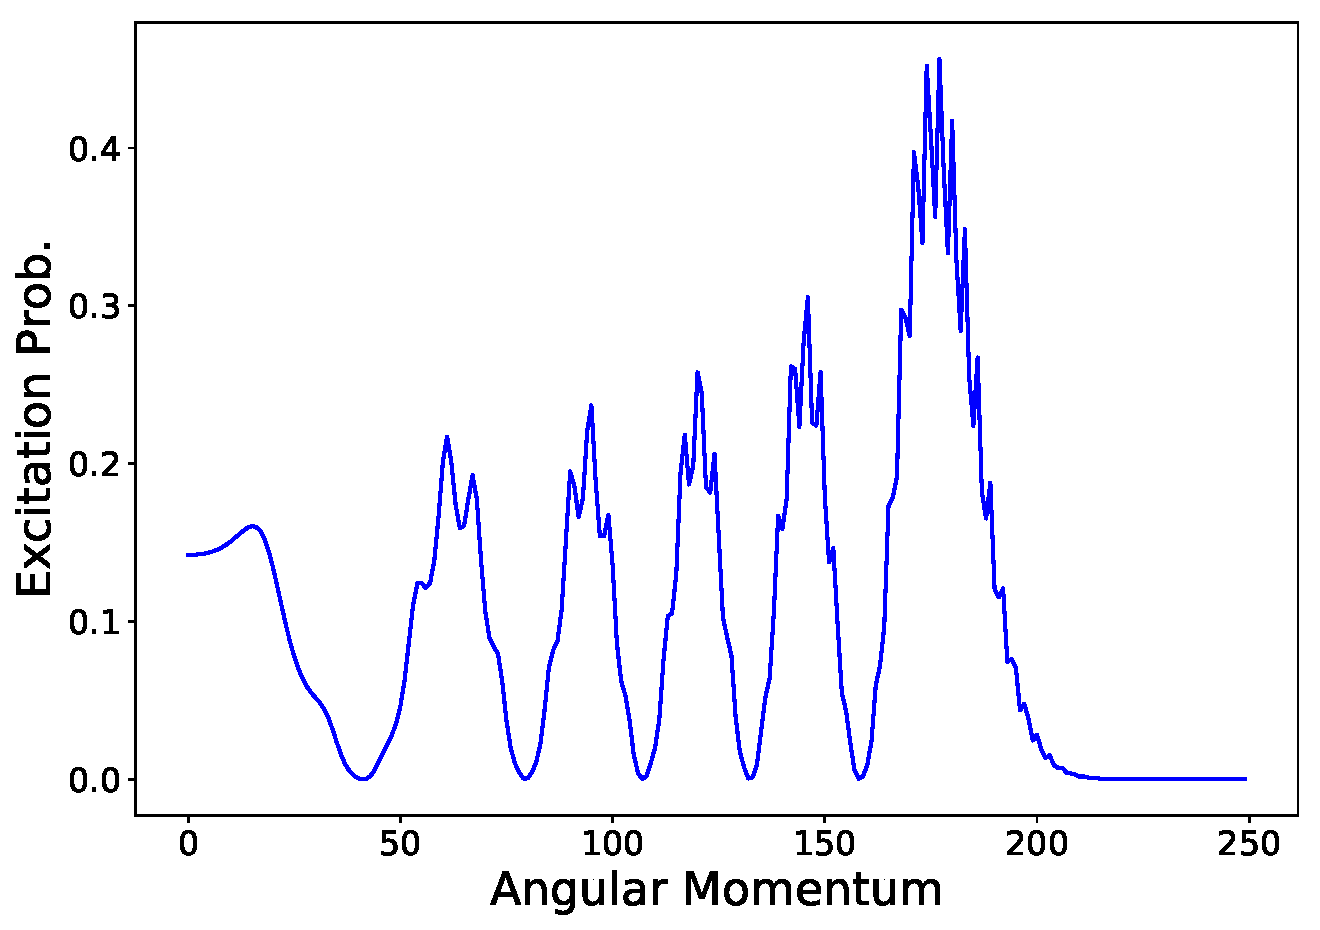
\includegraphics[width=1\columnwidth]{./Results/HeNeCollision}
%\caption{Excitation probability as a function of incoming angular momentum channel. The periodicity is set by the angular dependence of the excited state orbital as compared to incoming collision $\ell$, and the range of $\ell$ values covered is set by a competition between the collision energy and centrifugal barrier height.}
%\label{fig:HeNeCollision}
%\end{figure}
%
%Figure~\ref{fig:HeNeCollision} shows the excitation probability as a function of the incoming angular momentum $\ell$ of the collision complex. This has the expected shape when compared to experimental and theoretical studies of atom-ion collisions, e.g.~\cite{OlsonSmith71,}. The excitation probability oscillates due to the relative angular dependence of the incoming angular momentum and the orientation of the excited state atomic orbital. Due to the long-range nature of the Coulomb interaction, the peak excitation probability happens at very large incoming angular momenta which correspond to large impact parameters, which matches physical intuition for these sorts of atom-ion collisions.

\subsubsection{Atom-Atom Collisions}
We turn now to the collision between two neutral atoms. One is taken to be a structureless particle, for example a cold He atom present in buffer-gas cooling experiments conducted here at Harvard~\cite{Connolly2013,Tscherbul2010}. The other is assumed to be an alkaline-earth atom (e.g. Ca, Sr, etc.) with electron spin, which can be in either the ``spin-1" or ``spin-0" state. It is an experimental fact that particles with spin-1 can be magnetically trapped, while those with spin-0 cannot be. The trappable state is interesting because it can be held in an experiment for long times and studied spectroscopically. It is therefore an important problem to determine the probability that a collision will flip the spin of the atom, because this probability determines whether the atom can be stably trapped for experimentation. 

We use model interaction potentials $\mathbf{U}$ which are again represented in a $2 \times 2$ matrix because the only possible internal states correspond to the electron spin of the incoming alkali atom. It is customary to denote the interaction with the spin-0 atom by $V_\Sigma$ and the interaction with the spin-1 atom by $V_\Pi$. (The names come from the fact that the Greek letters $\Sigma$ and $\Pi$ generalize the letters $s$ and $p$ used to describe different atomic orbitals.) One extra energy term, denoted $A$ is the spin-orbit coupling energy and tells us how much energy is required to change the atom's spin state. In all, the interaction potential looks like:
\begin{equation}
\mathbf{U} = \left( \begin{array}{cc}
\frac{2}{3} V_\Sigma + \frac{1}{3} V_\Pi + A & \frac{\sqrt{2}}{3}(V_\Pi - V_\Sigma) \\
 \frac{\sqrt{2}}{3}(V_\Pi - V_\Sigma) & \frac{1}{3} V_\Sigma + \frac{2}{3} V_\Pi + 2A
\end{array} \right)
\end{equation}

\noindent where $V_i = C_{1,i} e^{-\lambda_{1,i} r} + (C_{2,i} + r C_{3,i}) e^{-\lambda_{2,i} r} - \frac{C_{4,i}}{2r^6}(\tanh( 1.2(r-\lambda_{3,i})+1)$ for $i = \Sigma, \Pi$ is a reasonable interaction potential model~\cite{Krems2017,Tscherbul2010,ColdChemBook}. We determine the constants by considering typical alkaline-earth atoms like Ca and Sr and then using the constants to fit potential wells describing their two lowest electronic spin states, using for instance data from~\cite{AlexanderNotes}. The constants chosen are listed in Tab.~\ref{tab:QuantumCoeffs} and $A$ is taken to be $3 \, \text{cm}^{-1}$. The diagonal terms, representing the energy states of the collision complex, come from the sum of these two potentials; off-diagonal terms, representing coupling between the states, is set by how anisotropic the interaction is and is therefore described by the different between these terms. The constants can then be determined via simple Clebsch-Gordan algebra for each total spin state and projection~\cite{Tscherbul2010,Connolloy2010}.

\begin{table}
\begin{center}
 \begin{tabular}{|c c c|} 
 \hline
 & $V_\Sigma$  & $V_\Pi$  \\
\hline\hline 
$C_1$ & 0.017 & -0.0354 \\ 
$C_2$ & 3.065 & -336.426 \\
$C_3$ & -0.5819 & 146.481 \\
$C_4$ & 15.82 & 13.5519 \\
$\lambda_1$ & 0.8 & 0.7 \\
$\lambda_2$ & 1.2 & 2.2 \\
$\lambda_3$ & 5.6&  6.21 \\
 \hline
\end{tabular}
\caption{Parameters used to describe the coupled-channels interaction potential. All are defined in atomic units.}
\label{tab:QuantumCoeffs}
\end{center}
\end {table}

We want to know the probability the spin will flip in a collision process, i.e. the total spin-flip inelastic \textit{integral cross-section} (ICS) denoted by $\sigma_{inel}$. This is defined by~\cite{Krems2017,ColdChemBook,ColdMolsBook} $\sigma_{inel} = \frac{\pi}{k^2} \sum_{\ell} (2\ell+1) \lvert S_{01} \rvert^2$. Hence, we first run the log-derivative code to determine the off-diagonal S-matrix element as a function of $\ell$. Then, depending on the collision energy we compute the inelastic cross-section by summing enough $\ell$ values at that energy to achieve convergence in the sum. We then repeat the process for a variety of energies to determine how the cross-section changes as a function of energy, or equivalently temperature. 

Physical intuition tells us a few things to expect. First, as the energy decreases, we will require fewer and fewer $\ell$ values to achieve convergence in the cross-section. This is because larger $\ell$ values give rise to larger centrifugal barriers $\sim \frac{\ell(\ell+1)}{r^2}$ in the potential energy, and as the collision energy decreases this centrifugal barrier effectively repels the colliding atom and prevents the collision from occurring. Eventually only the $\ell=0$ channel contributes, which physicists call ``single-partial-wave" scattering. Second, we expect that the inelastic cross-section will approach zero as the energy decreases, even in the single-partial-wave regime. This is because once the energy is much smaller than the typical scale of the coupling term, the interaction effectively decouples and cannot change the spin state. The range of parameters for which single-partial-wave scattering is achieved, and the range over which the inelastic cross-section becomes small, are both highly relevant experimentally because they set the temperatures above which stable trapping of the sample will become difficult. 

Now on to the numerical results. Figure~\ref{fig:AtomAtomVersusL} shows how the off-diagonal magnitude of the S-matrix behaves as a function of $\ell$ for a variety of collision energies. Clearly, as the collision energy increases more partial waves contribute, just as described above. We also plot, in Fig.~\ref{fig:AtomAtomVersusE}, the dependence of the off-diagonal S-matrix magnitude on collision energy for a variety of $\ell$ values. Again, matching the description of the centrifugal barrier, we see that larger $\ell$ values become prominent in the S-matrix only at sufficiently high energies. At low energies, below about $10$ K in this case, only the $\ell=0$ term contributes significantly. It is perhaps surprisingly that the spin-flip probability for $\ell = 0$ can be high for such low energies, but this is actually in agreement with calculations from the Wigner threshold laws~\cite{Krems2017,ColdMolsBook}. 

\begin{figure}[t]
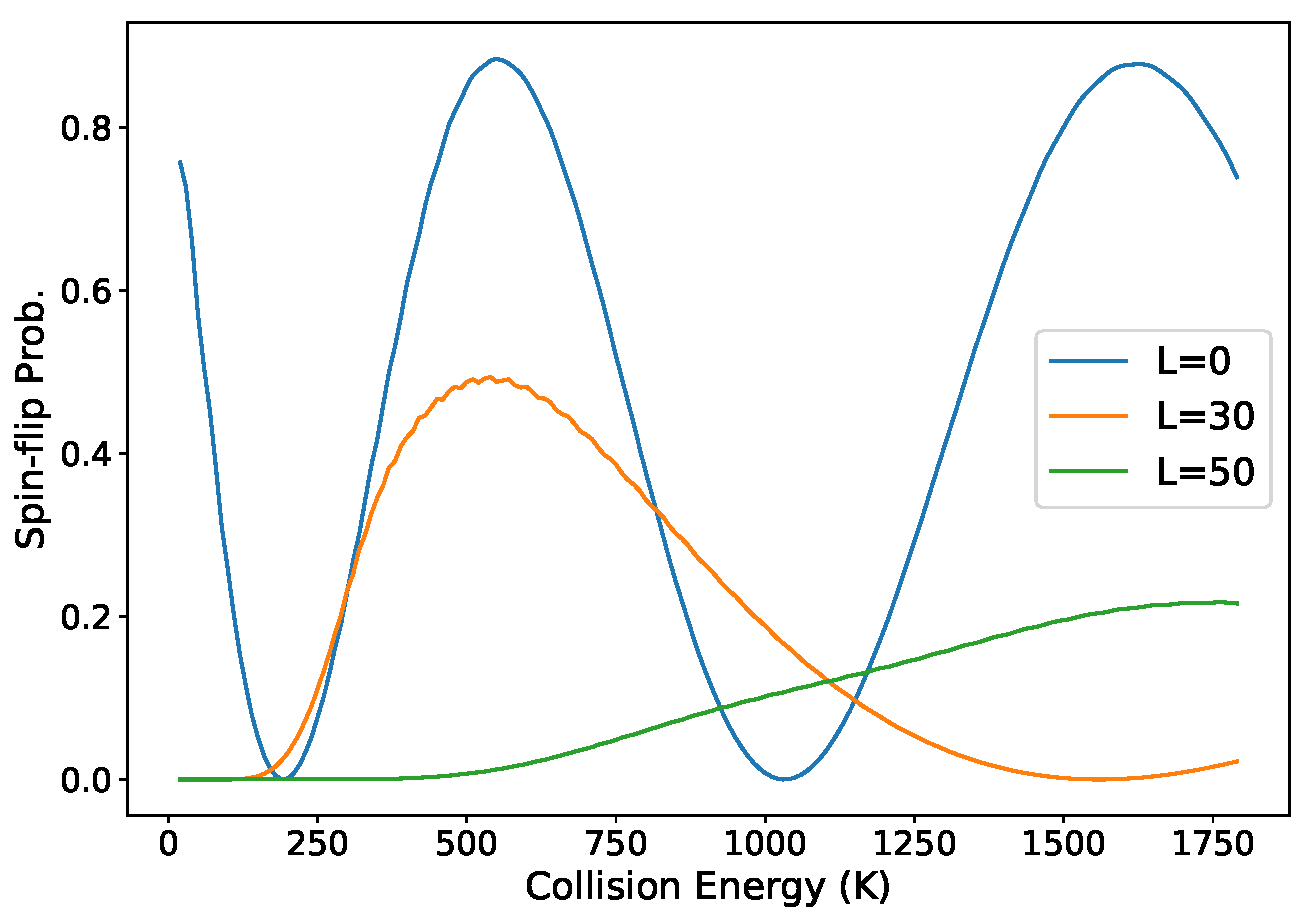
\includegraphics[width=1\columnwidth]{./Results/AtomAtomVersusE}
\caption{Spin-flip probability as a function of collision energy, for $\ell = 0, 30, 50$. The lowest energy plotted to $E = 20$ K. As the angular momentum increases, the centrifugal barrier increasingly suppresses the collision at that $\ell$.}
\label{fig:AtomAtomVersusE}
\end{figure}

\begin{figure}[b]
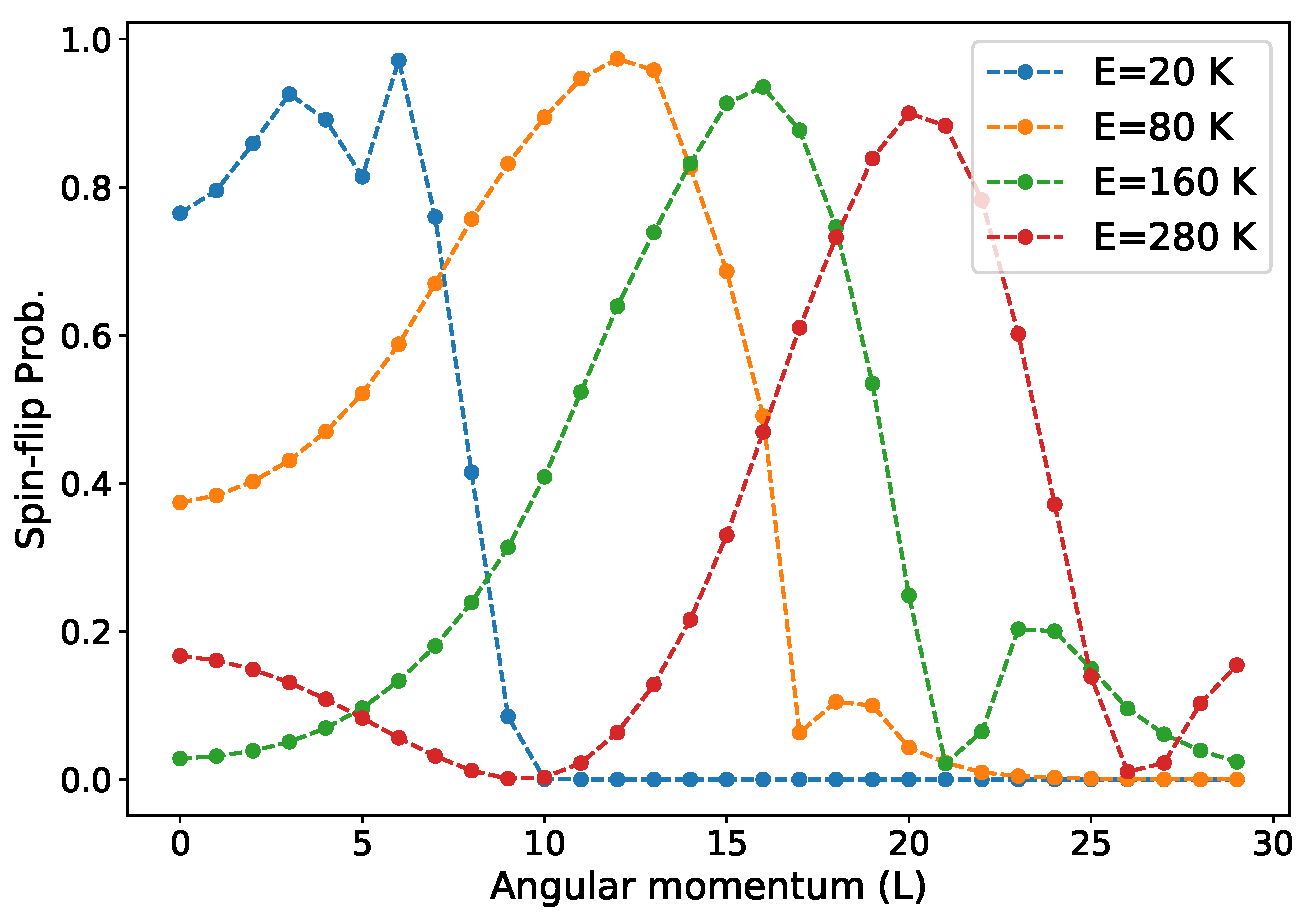
\includegraphics[width=1\columnwidth]{./Results/AtomAtomVersusL}
\caption{Spin-flip probability as a function of angular momentum channel, for a range of energies. As the collision energy increases, higher partial waves contribute more heavily because only these high energy collisions have energy to surpass the centrifugal barrier.}
\label{fig:AtomAtomVersusL}
\end{figure}

Finally, we can turn these S-matrix calculations into cross-sections and plot the total inelastic-cross section as a function of collision energy. Figure~\ref{fig:TotalCrossSection} shows the total inelastic cross section as a function of energy as well as the number of partial wave terms that contributed to the sum. Again, the simple physical reasoning provided above explains the behaviors: as the energy is decreased, the cross section falls and fewer partial waves contribute to the sum. We note that at temperatures of a few tens of K, the integral cross section begins to approach zero. This is easily explained by noting that the spin-orbit energy splitting constant assumed in the calculation was also of order 20 K ($3 \, \text{cm}^{-1} \approx 5 $ K). We would therefore expect spin-changing collisions to be negligible in exactly this regime. From an experimental perspective, then, it would appear that collisions between He atoms and alkaline-earth atoms like Ca and Sr should be robust against spin-changing losses at these cold temperatures. This is in qualitative agreement with the few experimental studies that have been undertaken in this parameter regime~\cite{Tscherbul2010,Connolly2013}.

\begin{figure}[t]
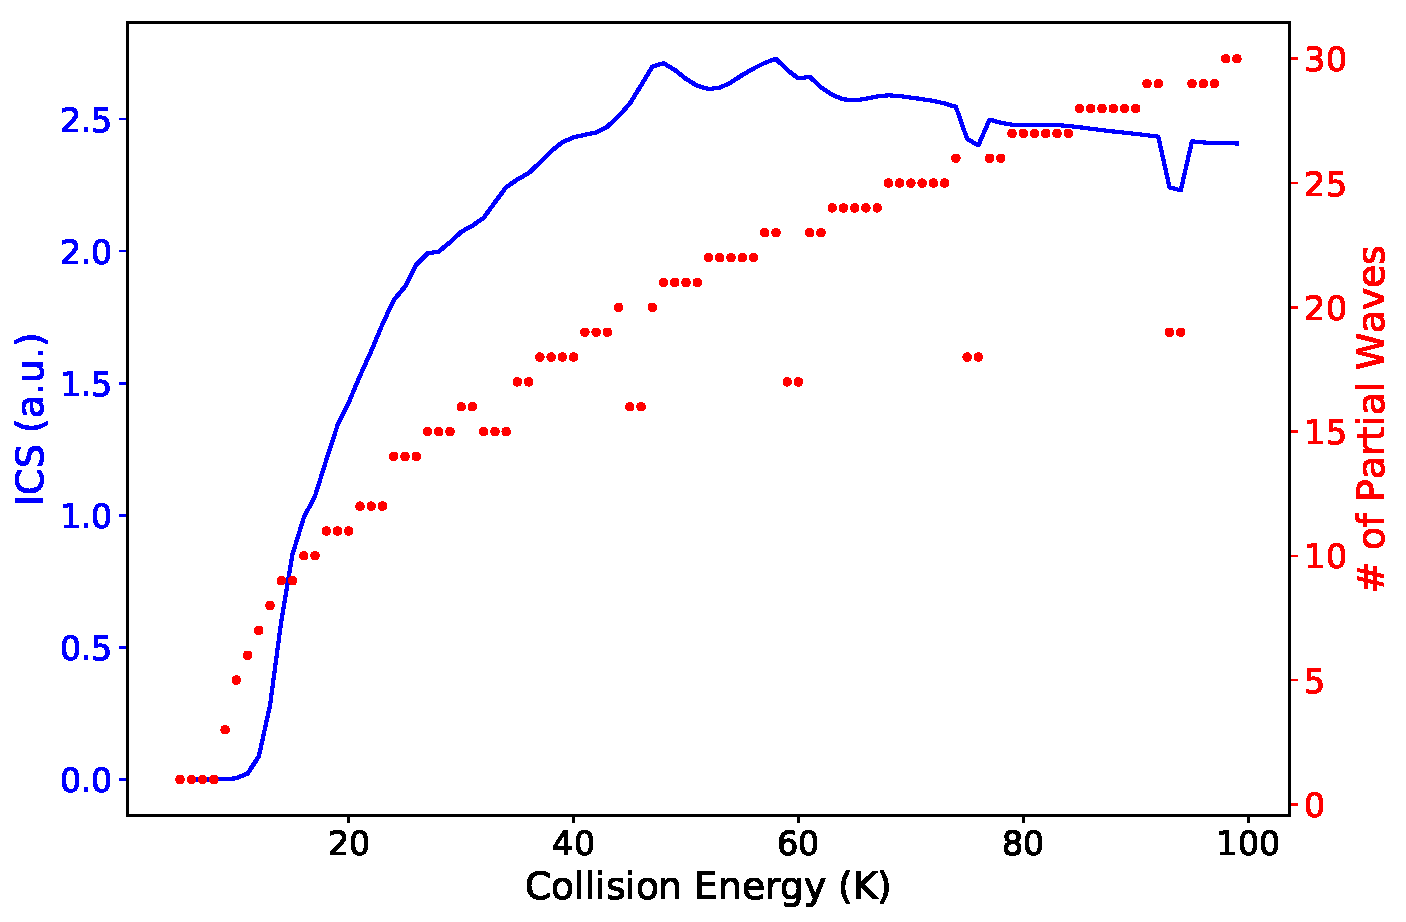
\includegraphics[width=1\columnwidth]{./Results/ICSandPartialWaves}
\caption{Total integral cross section (ICS) for the alkaline-earth atom - He collision complex. Also shown is the number of partial waves contributing to the scattering. At temperatures $\leq 20$ K, the integral cross section drops as do the number of partial waves required for the ICS sum to converge. Spin-changing collisions are expected to be negligible at these cold temperatures.}
\label{fig:TotalCrossSection}
\end{figure}

\section{Conclusion}
In summary, we have demonstrated three different methods for describing collisions between atoms and molecules. Our results have spanned purely classical to purely quantum mechanical theories. We have demonstrated the numerical methods with experimentally relevant simulations, focused mainly on the sorts of inelastic collisions which can lead to observable changes in the internal states of the colliding particles. From a classical perspective, we have investigated long-lived complexes formed from the intricate interactions between a colliding atom and a dimer. Quantum mechanically, we looked at state-changing inelastic collisions which could also lead to harmful trap loss from an experiment. 

There exist obvious immediate extensions to the work presented here. Foremost among these would be a quantum mechanical study of collisions involving more than two channels. Because our quantum simulations focused only on atom-atom collisions, we were able to restrict the problem to such a small number of channels: atoms have such sparse energy spectra, with such large energy gaps between the states, that collisions (especially at cold temperatures) are unlikely to couple more than a handful of channels. \textit{Molecular} collisions, on the other hand, require many more channels in an approximately complete basis because vibrational and rotational degrees of freedom give rise to rich forests of energy states with very small spacings. Therefore, this project could be developed further by running a full quantum calculation including these many channels. Indeed, the main limitation of our results is that the quantum mechanical description was limited to systems with a small number of incoming collision channels; more complex systems required us to resort to classical trajectory tracking.

Another possible continuation would be to compute accurate potential energy curves for an atom-atom collision complex. This would require \textit{ab initio} or semi-empirical formulas to describe the atomic structure and couplings between atomic states. A variety of methods and even some packages exist for this sort of computation~\cite{MOLPRO,Safronova}. In order to avoid the explosive growth of coupled channels, we could compute these for the same alkaline-earth atom + He collision considered above, where we had argued that only two collision channels needed to be considered. This would then allow us to test the accuracy of our potential energy curves by comparing against experimental data for a particular choice of atoms.

A simple estimate shows that, even at temperatures $\leq 1$ K, over 100 internal states would need to be included for molecules with small rotational and vibrational constants. Accurate potential energy surfaces would need to be developed to describe the coupling among these states, and then a large matrix problem would be solved over these potential energy curves. Importantly, the log-derivative method described above can easily be generalized to include these large matrix problems--- indeed, the code presented here was written to be fully general, and will adapt to any size interaction matrix $\mathbf{U}$. Given sufficiently accurate potential energy curves, it would be interesting to test the accuracy of the classical calculations presented here. One would expect based on Bohr's correspondence principle that at high energies, the classical results will hold. At lower energies, interesting quantum effects would be expected to arise. 

The field of ultracold atomic and molecular collisions is still, at least experimentally, in its infancy. Theoretical studies have so far outpaced experimental results due to the difficulty in producing samples of ultracold molecules. However, the past decade has seen tremendous progress on the experimental front and within the past two years, tens of species of ultracold molecules have been observed in the lab. A vibrant experiment-theory interplay can therefore be expected to grow stronger in the coming years: experimentalists can finally test the predictions of theorists, and theorists can continue pointing the way toward new and interesting physics. The future of atomic and molecular collisions is therefore quite bright.

\bibliography{WriteupFinal}% Produces the bibliography via BibTeX.

\end{document}
%
% ****** End of file apssamp.tex ******